\documentclass[        
    a4paper,          % Tamanho da folha A4
    12pt,             % Tamanho da fonte 12pt
    chapter=TITLE,    % Todos os capítulos devem ter caixa alta
    section=TITLE,    % Todas as seções devem ter caixa alta
    oneside,          % Usada para impressão em apenas uma face do papel
    english,          % Hifenizações em inglês
    spanish,          % Hifenizações em espanhol
    brazil            % Ultimo idioma eh o idioma padrão do documento
]{abntex2}

% Importações de pacotes
\usepackage[utf8]{inputenc}                         % Acentuação direta
\usepackage[T1]{fontenc}                            % Codificação da fonte em 8 bits
\usepackage{graphicx}                               % Inserir figuras
\usepackage{amsfonts, amssymb, amsmath}             % Fonte e símbolos matemáticos
\usepackage{booktabs}                               % Comandos para tabelas
\usepackage{verbatim}                               % Texto é interpretado como escrito no documento
\usepackage{multirow, array}                        % Múltiplas linhas e colunas em tabelas
\usepackage{indentfirst}                            % Endenta o primeiro parágrafo de cada seção.
\usepackage{listings}                               % Utilizar código fonte no documento
\usepackage{xcolor}
\usepackage{microtype}                              % Para melhorias de justificação?
\usepackage[portuguese,ruled,lined]{algorithm2e}    % Escrever algoritmos
\usepackage{algorithmic}                            % Criar Algoritmos  
\usepackage{amsgen}
\usepackage{lipsum}                                 % Usar a simulação de texto Lorem Ipsum
%\usepackage{titlesec}                               % Permite alterar os títulos do documento
\usepackage{tocloft}                                % Permite alterar a formatação do Sumário
\usepackage{etoolbox}                               % Usado para alterar a fonte da Section no Sumário
\usepackage[nogroupskip,nonumberlist,acronym]{glossaries}                % Permite fazer o glossário
\usepackage{caption}                                % Altera o comportamento da tag caption
\usepackage[alf, abnt-emphasize=bf, bibjustif, recuo=0cm, abnt-etal-cite=3, abnt-etal-list=0,abnt-etal-text=it]{abntex2cite}    % Citações padrão ABNT
%\usepackage[bottom]{footmisc}                      % Mantém as notas de rodapé sempre na mesma posição
%\usepackage{times}                                 % Usa a fonte Times
\usepackage{mathptmx}                               % Usa a fonte Times New Roman										
%\usepackage{lmodern}                                % Usa a fonte Latin Modern
%\usepackage{subfig}                                 % Posicionamento de figuras
%\usepackage{scalefnt}                               % Permite redimensionar tamanho da fonte
\usepackage{color, colortbl}                        % Comandos de cores
%\usepackage{lscape}                                 % Permite páginas em modo "paisagem"
%\usepackage{ae, aecompl}                            % Fontes de alta qualidade
%\usepackage{picinpar}                               % Dispor imagens em parágrafos
\usepackage{latexsym}                               % Símbolos matemáticos
%\usepackage{upgreek}                                % Fonte letras gregas
\usepackage{appendix}                               % Gerar o apêndice no final do documento
\usepackage{paracol}                                % Criar parágrafos sem identação
\usepackage{_lib/uniftex2}		                    % Biblioteca com as normas da Uniftec para trabalhos acadêmicos
\usepackage{pdfpages}                               % Incluir PDF no documento
\usepackage{amsmath}                                % Usar equações matemáticas
\usepackage{subcaption}                             % multi figures
\usepackage{float}                                  % Utilizado para criação de floats
\usepackage{pythonhighlight}
\usepackage{hyphenat}                               % Utilizado para criação de regras de hifenização

% Configuração fonte em legendas
\captionsetup{font={footnotesize, bf},labelfont={footnotesize, bf}}

% Fonte Arial
\usepackage{helvet}
\renewcommand{\familydefault}{\sfdefault}

% Organiza e gera a lista de abreviaturas, símbolos e glossário
\makeglossaries

% Gera o Índice do documento
\makeindex

%Habilita letras gregas sem usar o módulo math
\usepackage{textgreek}

\usepackage{tabulary}


%%%%%%%%%%%%%%%%%%%%%%%%%%%%%%%%%%%%%%%%%%%%%%%%%%%%%
%%          Configuracoes do ueceTeX2              %%
%%%%%%%%%%%%%%%%%%%%%%%%%%%%%%%%%%%%%%%%%%%%%%%%%%%%%

% Opcoes disponiveis

\trabalhoacademico{tccgraduacao}
%\trabalhoacademico{tccespecializacao}
%\trabalhoacademico{dissertacao}
%\trabalhoacademico{tese}

% Define se o trabalho eh uma qualificação
% Coloque 'nao' para versão final do trabalho

\ehqualificacao{nao}

% Remove as bordas vermelhas e verdes do PDF gerado
% Coloque 'sim' pare remover

\removerbordasdohyperlink{sim} 

% Adiciona a cor Azul a todos os hyperlinks

\cordohyperlink{nao}

%%%%%%%%%%%%%%%%%%%%%%%%%%%%%%%%%%%%%%%%%%%%%%%%%%%%%
%%          Informação sobre a IES                 %%
%%%%%%%%%%%%%%%%%%%%%%%%%%%%%%%%%%%%%%%%%%%%%%%%%%%%%

\ies{Centro Universitário Uniftec}
\iessigla{Uniftec}
\centro{Centro Universitário Uniftec}

%%%%%%%%%%%%%%%%%%%%%%%%%%%%%%%%%%%%%%%%%%%%%%%%%%%%%
%%        Informação para TCC de Graduação         %%
%%%%%%%%%%%%%%%%%%%%%%%%%%%%%%%%%%%%%%%%%%%%%%%%%%%%%

\graduacaoem{Engenharia de Computação}
% Pode colocar também 'licenciada'
\habilitacao{bacharel}

%%%%%%%%%%%%%%%%%%%%%%%%%%%%%%%%%%%%%%%%%%%%%%%%%%%%%
%%     Informação para TCC de Especialização       %%
%%%%%%%%%%%%%%%%%%%%%%%%%%%%%%%%%%%%%%%%%%%%%%%%%%%%%
\especializacaoem{Alfabetização de Crianças}

%%%%%%%%%%%%%%%%%%%%%%%%%%%%%%%%%%%%%%%%%%%%%%%%%%%%%
%%         Informação para Dissertação             %%
%%%%%%%%%%%%%%%%%%%%%%%%%%%%%%%%%%%%%%%%%%%%%%%%%%%%%
\programamestrado{Programa de Pós-Graduação em Ciência da Computação}
\nomedomestrado{Mestrado Acadêmico em Ciência da Computação}
\mestreem{Ciência da Computação}
\areadeconcentracaomestrado{Ciência da Computação}

%%%%%%%%%%%%%%%%%%%%%%%%%%%%%%%%%%%%%%%%%%%%%%%%%%%%%
%%               Informação para Tese              %%
%%%%%%%%%%%%%%%%%%%%%%%%%%%%%%%%%%%%%%%%%%%%%%%%%%%%%
\programadoutorado{Programa de Pós-Graduação em Saúde Coletiva}
\nomedodoutorado{Doutorado em Saúde Coletiva}
\doutorem{Saúde Coletiva}
\areadeconcentracaodoutorado{Saúde Coletiva}

%%%%%%%%%%%%%%%%%%%%%%%%%%%%%%%%%%%%%%%%%%%%%%
%%  Informação relacionadas ao trabalho     %%
%%%%%%%%%%%%%%%%%%%%%%%%%%%%%%%%%%%%%%%%%%%%%%
\autor{Vittoria Luiza da Silveira Thomasini}

\titulo{Identificação de Tom de Pele utilizando Inteligência Artificial para promover Diversidade e Inclusão na Indústria de Beleza} 

\data{2023}
\local{Caxias do Sul}

% Exemplo: \dataaprovacao{01 de Janeiro de 2012}
\dataaprovacao{}

%%%%%%%%%%%%%%%%%%%%%%%%%%%%%%%%%%%%%%%%%%%%%
%%     Informação sobre o Orientador       %%
%%%%%%%%%%%%%%%%%%%%%%%%%%%%%%%%%%%%%%%%%%%%%
\orientador{João Luis Tavares}
\orientadories{Centro Universitário Uniftec – Uniftec}
\orientadorcentro{Centro Universitário Uniftec – Uniftec}
\orientadorfeminino{nao} % Coloque 'sim' se for do sexo feminino

%%%%%%%%%%%%%%%%%%%%%%%%%%%%%%%%%%%%%%%%%%%%%
%%      Informação sobre o Co-orientador   %%
%%%%%%%%%%%%%%%%%%%%%%%%%%%%%%%%%%%%%%%%%%%%%

% Deixe o nome do coorientador em branco para remover do documento
\coorientador{}
\coorientadories{Universidade Co-orientador - SIGLA}
\coorientadorcentro{Centro do Co-orientador - SIGLA}
\coorientadorfeminino{nao} % Coloque 'sim' se for do sexo feminino

%%%%%%%%%%%%%%%%%%%%%%%%%%%%%%%%%%%%%%%%%%%%%
%%      Informação sobre a banca           %%
%%%%%%%%%%%%%%%%%%%%%%%%%%%%%%%%%%%%%%%%%%%%%

% Atenção! Deixe o nome do membro da banca para remover da folha de aprovação

% Exemplo de uso:
% \membrodabancadois{Prof. Dr. Fulano de Tal}
% \membrodabancadoisies{Universidade Estadual do Ceará - UECE}

\membrodabancadois{Membro da Banca Dois}
\membrodabancadoiscentro{Centro do Membro da Banca Dois - SIGLA}
\membrodabancadoisies{Universidade do Membro da Banca Dois - SIGLA}
\membrodabancatres{Membro da Banca Tres - SIGLA}
\membrodabancatrescentro{Centro do Membro da Banca Tres - SIGLA}
\membrodabancatresies{Universidade do Membro da Banca Três - SIGLA}
\membrodabancaquatro{Membro da Banca Quatro - SIGLA}
\membrodabancaquatrocentro{Centro do Membro da Banca Quatro - SIGLA}
\membrodabancaquatroies{Universidade do Membro da Banca Quatro - SIGLA}
\membrodabancacinco{Membro da Banca Cinco}
\membrodabancacincocentro{Teste}
\membrodabancacincoies{Universidade do Membro da Banca Cinco - SIGLA}
\membrodabancaseis{Membro da Banca Seis}
\membrodabancaseiscentro{}
\membrodabancaseisies{Universidade do Membro da Banca Seis - SIGLA}

\begin{document}
    % Elementos pré-textuais
    \pretextual
	\imprimircapa
	\imprimirfolhaderosto{}
%%	\imprimirfichacatalografica{elementos-pre-textuais/ficha-catalografica}
%%	\imprimirerrata{elementos-pre-textuais/errata}
	\imprimirfolhadeaprovacao
%%	\imprimirdedicatoria{elementos-pre-textuais/dedicatoria}
%%	\imprimiragradecimentos{elementos-pre-textuais/agradecimentos}
%%	\imprimirepigrafe{elementos-pre-textuais/epigrafe}
	\imprimirresumo{elementos-pre-textuais/resumo}
	\imprimirabstract{elementos-pre-textuais/abstract}
	\imprimirlistadeilustracoes
	\imprimirlistadetabelas
	\imprimirlistadequadros
	\imprimirlistadealgoritmos
%%	\imprimirlistadecodigosfonte
	\imprimirlistadeabreviaturasesiglas
	\imprimirlistadesimbolos{elementos-pre-textuais/lista-de-simbolos}   
	\imprimirsumario

    % Elementos textuais	
    \textual
    \chapter{Introdução}
\label{cap:introducao}

A indústria de cosméticos do Brasil é uma das maiores do mercado de cosméticos mundial, sendo em 2022 responsável por exportar mais de 770 milhões de dólares em produtos de beleza e higiene\cite{Cosmetics_industry_in_Brazil}. A maquiagem além de uma arte corporal que já é utilizada a mais de 7000 anos também tem impacto pessoal e social a vida de quem o usa e das pessoas ao redor. Muitas vezes, a maquiagem é usada na intenção de realçar a beleza, onde pode gerar um efeito sobre a atratividade facial, corrigindo imperfeições e realçando características. Além disso, pode estar associada com maiores atribuições de sucesso profissional, renda salarial e posição socioeconômico \cite{Respostas_Emocionais_Implícitas_Julgamento_da_Atratividade_Facial_em_Faces}.

 Nessa indústria, a cor é uma característica chave para os consumidores e  fabricantes de cosméticos. E, entre os cosméticos disponíveis no mercado, encontrar a base que combina com a cor da pele pode ser decisivo para um bom acabamento. Contudo, diferentes marcas desenvolvem diferentes cartelas de cores, para tipos de pele diferentes e tipos acabamentos, resultando em inúmeras opções de bases disponíveis no mercado. Isso sem considerar que as marcas no segmento de beleza podem ser categorizada de por tipos diferentes de produtos como sendo naturais, urbano, jovem, orgânicos, veganos, \textit{cruelty free}, limpos e entre outros. Por isso, embora haja opções disponíveis, também há a dificuldade do cliente em encontrar o tom que o atenda. Principalmente em um país de grande miscigenação como Brasil, onde podemos encontrar todos os fotótipos Fitzpatrick espelhados pelo país e diferentes variações.\cite{Régua_de_Pele_Linha_de_Maquiagem_para_a_Mulher_Brasileira}

Segundo o artigo \cite{Snap_and_match_a_case_study_of_virtual_color_cosmetics_consultation} foi conduzido pela empresa Estée Lauder um estudo online que apontou que 70\% das mulheres não conseguem encontrar o tom exato que combina com a cor da pele e que 94\% das mulheres estão usando a cor errada da base. Isso pode ocorrer porque muitas mulheres brasileiras por serem muito brancas categorizadas como fototipo I, morenas escuras como fototipo V, e  negras, fototipo VI\cite{Régua_de_Pele_Linha_de_Maquiagem_para_a_Mulher_Brasileira}.
A maneira tradicional do consumidor de determinar qual a base de cor combina com a pele requer aplicar tons disponíveis na loja na pele \cite{A_development_of_a_portable_device_for_skin_color_estimation_on_cosmetic_foundation_applying} ou por seleção visual, sendo a compra também em loja virtual ou com a ajuda de vendedores em uma loja \cite{Snap_and_match_a_case_study_of_virtual_color_cosmetics_consultation}.
E, no mercado profissional, os maquiadores misturam dois ou mais tons de base para encontrar a cor ideal da cliente. Contudo, dependendo das condições de iluminação, pode levar a uma aparência não natural comparado a outra condição de iluminação.  Isso pode ser causado principalmente por problemas ópticos, já que espectros da pele podem ser bem diferentes dos das bases cosméticas. Assim, como a escolha da região de teste pode ter diferença de coloração com a região de uso, como, por exemplo, testar no braço ou pescoço o tom, sendo que o produto será utilizado para uniformizar a coloração facial. Nesse caso, a ajuda ao consumidor na hora da escolha pode ser uma estratégia para fidelizar o cliente.
Nesse sentido, empresas de cosméticos apostam em serviços personalizados usando principalmente da realidade virtual, a realidade aumentada e a consultoria para auxiliar o consumidor na escolha de seus produtos.



    \section{Justificativa}
\label{justificativa}

A motivação para o desenvolvimento do trabalho reside na problemática de muitos consumidores terem dificuldades em identificar o próprio tom de pele e conseguir identificar no mercado de cosméticos um produto que tenha um tom que combine com o seu. Atualmente, muito se fala de diversidade e inclusão na indústria de cosméticos e por isso cada vez mais marcas estão desenvolvendo cartelas com faixas de cores mais amplas.

No mercado de varejo entende-se que estratégias que auxiliam os clientes a executarem tarefas que entregam valor e reconhecimento pessoal são mais eficazes para fidelizar o cliente \cite{Snap_and_match_a_case_study_of_virtual_color_cosmetics_consultation}, por isso, pensando nisso e com a crescente demanda de personalização, com a tecnologia tornando-se uma ferramenta a fim de estimular a experiência dos consumidores. Surgiu a ideia do projeto de desenvolvimento utilizando técnicas de inteligência artificial para identificar e classificar o tom de pele para auxiliar os consumidores a identificarem o seu próprio tom de pele. 

Existem diversas abordagens para detecção de pele, mas poucos estudos que se dedicam a estudar tons de pele em si. Maior parte dos estudos se dedicam a averiguar melhores abordagens para detecção de pele voltada ao reconhecimento facial. Por isso, para o desenvolvimento do trabalho buscou se focar na identificação com menos interferências possíveis de iluminação e fundo, assim como a influência a região dos olhos, boca, nariz e cabelos. Por isso precisou-se de uma avaliação e comparação entre técnicas a serem utilizadas. Este trabalho foi realizado para realizar a avaliação e de propor uma aplicação de detecção de tom de pele que atenda os seguintes requisitos: precisão e desempenho.

O requisito de precisão para ser possível a utilização de fotos sem ambiente controlado de iluminação e qualidade de imagem. Dessa forma, o sistema deverá detectar o tom de pele humana em imagens com iluminações inadequadas, com o mínimo de interferência de fundo e com variadas resoluções. Além disso, o requisito de desempenho para que o sistema que utilize o programa de identificação e classificação processe as imagens em tempo real, sendo possível o cliente tirar a própria foto e já possuir o resultado da avaliação.

Além disso, diversas aplicações poderão usar os resultados da detecção e classificação de tom de pele, principalmente voltado a indústria da beleza, por profissionais da área de visagismo, maquiadores, pesquisadores sociais, entre outros.

\chapter{Objetivos}
Com o propósito de identificar subtons de pele utilizando técnicas de inteligência artificial, foram estabelecidos alguns objetivos descritos nesta seção. A Seção~\ref{objetivosgerais} apresenta o objetivo principal do trabalho, enquanto a Seção~\ref{objetivosespecificos} detalha os objetivos específicos e por fim a seção~\ref{justificativa} apresenta as justificativas que motivaram o desenvolvimento deste estudo.

\section{Objetivos Gerais}
\label{objetivosgerais}

O objetivo principal deste trabalho é detectar e identificar tons e subtons de pele humana em imagens, utilizando a escala \textit{Monk Skin Tone}(CITAÇÃO) como métrica de classificação, com o intuito de sugerir melhores formulações de cartela de cores para futuras aplicações de recomendação de produtos de maquiagem.
\section{Objetivos Específicos}
\label{objetivosespecificos}

Para o objetivo principal poder ser obtido, os seguintes objetivos específicos foram propostos:

\begin{itemize}
    \item[--] Realizar uma pesquisa bibliográfica sobre o tema proposto;
    \item[--] Identificar a técnica adequada de\textsl{Machine Learning} a ser aplicada;
    \item[--] Obter e tratar as imagens utilizando a biblioteca de manipulação de imagens OpenCV;
    \item[--] Segmentar as imagens para extrair informações da imagem relevantes para classificação de tons da pele; 
    \item[--] Desenvolver algoritmos de identificação da escala de tons a partir da extração da cor dominante da pele;
    \item[--] Classificar o tom dominante identificado conforme a paleta de Monk; 
    \item[--] Validar a classificação do tom dominante identificado conforme a paleta de Monk; 
\end{itemize}
    \chapter{Referencial Teórico}
Este capítulo apresenta os principais conceitos explorados para o desenvolvimento do presente trabalho, cobrindo as tecnologias necessárias e os conceitos imprescindíveis para a construção da proposta e o estudo para o desenvolvimento do projeto. Com o intuito de fundamentar a metodologia, foram estudados os conceitos e características do visagismo, grupos de pele, características e grupos cromáticos de pele, escalas de tons. Em seguida são apresentados os conceitos e técnicas de processamento digital de imagens relacionadas ao sistema de cores, técnicas de classificação automática e tratamento digital de imagens.

A percepção visual da cor da pele desempenha impacto importante no papel social de um indivíduo perante a avaliação de etnia, idade, saúde \cite{Classification_Algorithm_for_Skin_Color_CASCo_A_new_tool} e atratividade \cite{Respostas_Emocionais_Implícitas_Julgamento_da_Atratividade_Facial_em_Faces}. A cor da pele do indivíduo pode ser interpretada como indicador de sua história, decorrente da sua inserção em determinado grupo social \cite{Color_criteria_of_facial_skin_tone_judgment}. Sendo assim, ela não só configura o fator genético, mas também o fator sociocultural que influencia no modo que o indivíduo consome. O que pode alterar a percepção individual e as suas preferências de produtos entre os usuários de maquiagem, especialmente na escolha de maquiagens, como pelo valor do produto, acabamento e o tom de base a ser utilizado.

Nos países asiáticos, como o Japão, o padrão de beleza é a pele clara, onde é comum a venda de produtos que clareiam e protegem a pele contra raios UV (Ultravioleta), pois a pele branca é tratada como nobre. Já em países ocidentais tem se tornado comum a discussão de representatividade, principalmente da pele preta. No Brasil e Estados Unidos, as marcas vem abordando o mercado com novos produtos que possuem faixas de cores mais abrangentes. Como a empresa Fenty Beauty\footnote{https://fentybeauty.com/} que se destacou no mercado por ter seu primeiro lançamento de 50 tons de base e a empresa Bruna Tavares\footnote{https://www.linhabrunatavares.com/}, no Brasil, quando seu primeiro lançamento continha 30 tons, algo revolucionário para o mercado. Porém, além do problema das cartelas de cores, há a falta de padronização na nomenclatura para as cores, dificultando para o consumidor encontrar uma mesma cor em diferentes marcas.

A base pode ser líquida, em pó ou creme e é o primeiro passo na maquiagem facial.  E são utilizadas para deixar a pele uniformizada, cobrindo manchas, alterando o tom e a textura para a impressão de uma pele mais saudável e jovem \footnote{https://www.cosmeticsinfo.org/products/foundations/}. O tom de base é parte fundamental de uma maquiagem que pode ou não criar um efeito máscara no cliente devido à discrepância de coloração de pele que pode gerar entre o corpo e face.

A escolha do tom de um produto, como a base, pode ser alterada conforme o tom e subtom de pele que a pessoa possui. Isso se deve a tonalidade do produto impactar a percepção e compatibilidade de acabamento entre a pele e o produto, que se não semelhante ou igual transmite efeitos indesejados como estranheza pela distinção entre áreas de rosto, colo e pescoço. 
%Por isso, a escolha de não só um tom semelhante à pele, mas o subtom do produto, sendo ele quente, frio ou neutro, impacta a imagem a ser transmitida e elas devem ser avaliadas separadamente. 
Por isso é importante a escolha de um tom semelhante à pele e também do subtom do produto (quente, frio ou neutro), impactando a imagem a ser transmitida que deve ser avaliada separadamente.
De acordo com \cite{Maquiagem_técnicas_referências_e_atuação_profissional}  o  subtom  não tem relação com o tom de pele nem a etnia, mas as substâncias como a \textit{melanina}. A melanina é dividida em duas substâncias, sendo elas a \textit{fenomelanina} que dá pigmentação amarelada e avermelhada à pele e a \textit{eumelanina} que acentua tons marrons e pretos.

\section{Visagismo}
O visagismo foi criado por Fernand Aubry em 1937 e tem origem do termo \textit{visagisme}, palavra que, em francês, significa rosto. Contudo, Fernand Aubry não definiu o conceito do visagismo. Entendeu-se a partir de fragmentos de suas aulas de maquiagem que ele acreditava que o profissional de beleza deveria criar em seus clientes uma imagem harmônica e equilibrada visualmente e que essa imagem deveria expressar uma personalidade \cite{Visagismo_Harmonia_e_Estetica}.

O visagismo foi introduzido no Brasil a partir do livro de Philip Hallawell, que define como a técnica que compõe a imagem pessoal, revelando as qualidades de uma pessoa conforme as suas características físicas e princípios da linguagem visual que se deseja expressar. Essa técnica promove a arte visual, propondo uma relação entre emoções e personalidade, com foco na construção da imagem e beleza \cite{Visagismo_Harmonia_e_Estetica}. Assim, a técnica permite que os profissionais da beleza utilizem do seu conhecimento técnico para auxiliar o seu cliente a definir e se expressar através da sua imagem. Além disso, o conceito do visagismo surge para acabar com a padronização do conceito de beleza\cite{Visagismo}. 

\subsection{Caracterização cromática de pele}
O rosto é o local onde as pessoas se identificam, e qualquer alteração na sua aparência pode alterar essa identificação. Por isso, a relevância do visagismo, pois mudanças na aparência podem influenciar negativamente na vida profissional ou pessoal do indivíduo, assim como o uso ou não de maquiagens \cite{Respostas_Emocionais_Implícitas_Julgamento_da_Atratividade_Facial_em_Faces}. No caso da análise da cor da pele, a coloração pessoal, no visagismo, busca-se identificar as cores que harmonizam com a pele e a realçam com o subtom de pele de cada
pessoa \cite{A_influencia_da_coloração_pessoal_na_autoestima_e_autoimagem}. Para isso, são analisadas as cores superficiais e a temperatura da pele. A cor superficial nas peles brancas se refere ao tom amarelado ou avermelhado; e nas peles negras, amarelado, avermelhado ou marrom-escuro. Para a temperatura da pele existem as cores quentes como o laranja, amarelo e vermelho-alaranjado ou vermelho cádmio e frias, como o magenta, roxo, verde e azul. \cite{Visagismo}. Além disso, há a possibilidade de harmonizar a pele fria com a cor prateada e peles quentes com a cor dourada. Assim como pode ser analisado, as veias do antebraço apresentarem tonalidades verde ou amarelada, sendo a pele  quente e se manifestarem o azul ou rosada o tom é frio. 

Segundo \cite{Visagismo}, para se definir a cor de pele é preciso identificar o tom de pele, sendo ela clara ou escura. Algumas peles negras podem ser confundidas com peles brancas, mas possuem características bem distintas. Em seguida, a temperatura da pele deve se aproximar de uma amostra de cor bege e outra branca, onde peles quentes combinam com a cor bege, enquanto as peles frias combinam com branco e peles neutras combinam com ambas as cores. E,  finalmente, a estação da pele, no qual a classificação de cada tonalidade de pele é baseada em estações e dividida entre peles brancas e negras.

\subsection{Grupos cromáticos}
Para a coloração pessoal no visagismo existe uma classificação das cores da pele com referências às estações do ano, pois todas as peles se identificavam com as cores da natureza e nela estão presentes as cores frias e quentes. De acordo com \cite{Visagismo_Harmonia_e_Estetica}, há quatro classificações para tons de pele, sendo elas primavera, outono, inverno e verão. Na classificação de peles quentes temos, consoante as estações do ano, a primavera e outono, e para peles frias, as estações de verão e inverno. Na análise de coloração pessoal também são consideradas a coloração de cabelo e de olhos e seu realce quando comparados com outras tonalidades, sendo elas proveniente de roupas, acessórios ou mesmo da maquiagem utilizada.

%Para as categorias quentes a classificação da primavera as tonalidades de pele, o tom de pele básico é o dourado amarelado e quando se expõe ao sol, produz um bronzeado dourado. 
Na classificação primavera para as tonalidades de pele, a categoria quente aponta para o tom de pele básico, que é o dourado amarelado e, quando exposto ao sol, produz um bronzeado dourado.
Para a pele outono há a classificação dos avermelhados. As pessoas mais claras que possuem esse tipo de pele, quando se expõem ao sol, se queimam facilmente, mas é raro que consigam se bronzear. As pessoas com a tonalidade mais escura ficam com um bronzeado acobreado. Existem dois tipos da pele outono: a pele mais clara e mais escura. 

Para as categorias frias a classificação do tipo inverno são frias e de categoria amareladas, podendo ter o fundo roxo. São opacas, pálidas e, quando se expõem ao sol, ficam com o tipo de bronzeado café, porém, podem escurecer, ficar manchadas e não absorver a cor. As peles do tipo verão são frias, mais delicadas e tendem a ser rosadas com o fundo azulado. Quando se expõem ao sol, queimam com facilidade, porém, não se bronzeiam, têm o bronzeado neutro. 

As peles negras também são muito variadas, vão desde as mais claras, sendo acinzentadas, amareladas, às escuras, sendo avermelhadas, e as muito escuras, sendo azuladas. Podem ser classificadas em tipos frios e quentes. Peles negras contêm muitas cores na sua composição, além da cor de base por serem mais escuras, as peles negras não miscigenadas têm pouco, ou nada, de branco. Todas as peles negras derivam do marrom, variando entre tons de dourado até os tons azulados. Em pessoas com a tonalidade de pele mais clara, existe mais branco, o que pode resultar em um tom neutro ou mais acinzentado. Para a pele negra são classificadas em tonalidades Nilo, Jazz, Saara, Calipso e Spike.

O tipo Nilo se refere a tonalidade neutra da pele e tende a ser uma coloração fria, mais claro e aproximando-se da cor de marfim. O fundo é azul-claro cinzento, porém não tem semelhanças com a pele verão. As peles negras da tonalidade Blues têm o fundo azul, muito escuras e frias. O tipo de pele jazz é escuro, da cor de chocolate ou café, porém mais claro que o tipo blues. Seu fundo é o verde, o que o torna frio. Já o tom Saara tem como característica a cor amarelada clara neutra. Pode parecer com algumas peles do tipo inverno, já que tem o fundo roxo. A pele do tipo calipso tem tonalidade dourada, quente e com fundo terra de siena natural, que se assemelha à pele primavera mais escura. Essa cor de pele é luminosa, vibrante e de tom médio. Tem características de cores quentes e parece estar bronzeada todo o tempo. E, a pele do tipo Spike, têm fundo verde terra, são uma pele avermelhada e se assemelham ao tipo de peles mais escuras, como o tipo outono \cite{Visagismo}. 


\section{Escalas de Tom de Pele}
O termo “cor da pele” geralmente refletem considerações étnicas. Por isso, o termo “tom de pele” para se  referir apenas à percepção precisa da cor da pele facial humana\cite{Color_criteria_of_facial_skin_tone_judgment}.

A cor de pele está relacionada a pigmentação herdada geneticamente e da cor induzida pela exposição solar. Para seu estudo há diversas classificações e escalas de tom de pele que se referem a tonalidades agrupadas de acordo com certas características como: sensibilidade a luz ultravioleta, região geográfica e etnia. A seguir, serão abordadas as principais escalas presentes no trabalho.


\subsection{Escala de Fitzpatrick}
A escala de Fitzpatrick é uma ferramenta dermatológica reconhecida internacionalmente para classificação do tipo de pele e sua sensibilidade à radiação ultravioleta. Esta escala de classificação originou-se em 1975 desenvolvida pelo médico dermatologista Thomas B. Fitzpatrick e  utiliza seis classes de cores de pele para descrever o comportamento da pele pelo bronzeamento. Conforme a Figura \ref{fig:x fototipo_fitzpatrick},  por exemplo,  o  Tipo  I  é  para  a  pele  muito  clara, que sofre queimaduras e não se  bronzeia, enquanto   o   Tipo   VI,   corresponde   à pele negra que  não sofre queimaduras  e  sempre  se bronzeia por conta da presença maior de melanina \cite{Fitzpatrick_1988}. Contudo, apesar de ser uma escala aceita amplamente na comunidade de dermatologia, essa escala necessita de treinamento e, por vezes, é considerada subjetiva, já essencialmente se baseia em uma análise empírica a partir da observação \cite{Classificao_de_fototipos_de_pele}.

\begin{figure}[h]
\caption{Fotótipos de Fitzpatrick}
\centering

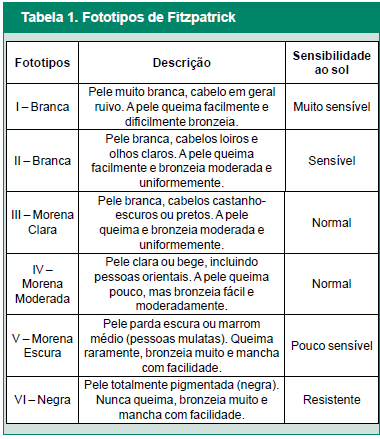
\includegraphics[]{Template_Latex_TCC-UNIFTEC/_lib/imagens/fototipo.png}

\label{fig:x fototipo_fitzpatrick}
\centering{\Fonte{\cite{Régua_de_Pele_Linha_de_Maquiagem_para_a_Mulher_Brasileira}.}}
\end{figure}

Segundo a Sociedade Brasileira de Dermatologia (SBD)\cite{Classificacao-dos-fototipos-de-pele-SBD}, a escala tem aplicabilidade para questões técnico-científicas, como a elaboração do planejamento para tratamento de fototerapia. Contudo, a escala de Fitzpatrick baseia-se, originalmente, na resposta da radiação violeta à pele branca \cite{Classificao_de_fototipos_de_pele} e para o desenvolvimento de \textit{machine learning} ela resultou em viés não intencional que exclui tons mais escuros \cite{Monk_2019}.
 

\subsection{Escala de Monk}
A pesquisa envolta no desenvolvimento da escala de Monk (MST - \textit{Monk Skin Tone}) tem como um dos objetivos tornar a visão computacional mais inclusiva. A paleta foi criada para substituir o padrão falho das seis cores de Fitzpatrick \cite{Monk_2019}, que, até o momento, é o padrão da indústria de tecnologia para categorizar o tom de pele. Criada pelo Dr. Ellis Monk essa paleta está sendo usada pela empresa Google para promover diversidade e inclusão na tecnologia. Ela fornece um espectro mais amplo de tons de pele que pode ser aproveitado para avaliar conjuntos de dados e modelos de \textit{machine learning} para melhor representação.

A paleta foi desenvolvida com base na pesquisa do Dr. Monk sobre os tons de pele e estudo de colorismo nos Estados Unidos e Brasil, que se concentrava em estudar a variação da exposição geográfica à radiação ultravioleta cria diferentes distribuições de tons de pele entre as populações. A paleta foi avaliada por especialistas em psicologia social e categorização social, bem como comunidades sub-representadas, para saber como eles percebiam a escala. Resulta em uma escala de 10 tons projetada para representar uma gama maior das comunidades \cite{Monk_2019}.

Recentemente a paleta foi validada como sendo mais inclusiva e com melhor representatividade de tons de pele do que a escala de Fitzpatrick para fins de treinamento de ML \cite{Monk_2019}. Além disso, também foi avaliado que a escala de Monk é tão representativa quanto uma paleta de beleza de 40 cores \cite{Monk_2019}. As escalas de tom de base de empresas de maquiagem podem incluir mais de 40 tons de pele, isso sem considerar diferenças de tons de produto entre linhas da mesma marca. Porém, quanto maiores as escalas, maior o desafio para casos de uso de ML, devido à dificuldade de aplicar tantos tons consistentemente em uma ampla variedade de conteúdo \cite{Monk_2019}. No caso da classificação do tom de pele, o problema passa a ser mais difícil. Quanto mais tons são agregados com parâmetros, mais próximos e semelhantes há impacto na classificação \cite{Automatic_Skin_Tone_Extraction_for_Visagism_Applications}.Sendo assim, os 10 tons possuem granularidade suficiente para refletir uma diversidade de comunidades, sem aumentar a complexidade, permitindo treinamento e avaliação de ML. É importante salientar, que a paleta não planeja identificar uma cor exata de pele, uma vez que a cor da pele humana é extremamente variável e complexa. Ao contrário, o objetivo é assegurar que os pesquisadores possam ver uma medida de tom de pele e encontrar um tom mais próximo.

\section{Tipos de pele brasileira}
O Brasil é um país conhecido por ser miscigenado e por conta disso possui inúmeros tipos de tons de pele. Segundo o \cite{ibge_2022}, na Pesquisa Nacional por Amostra de Domicílios (PNAD) Contínua, 42,8\% dos brasileiros se declararam como brancos, 45,3\% como pardos e 10,6\% como pretos. Não há dados que indiquem qual a tonalidade dos pesquisados, contudo, o Grupo Boticário realizou um estudo que indicou a existência de 168 tons de pele no Brasil, sendo 32 delas correspondentes a 98\% da população \cite{168_tons}, essas informações foram utilizadas para o desenvolvimento de novas cartelas de cores para o grupo atender. 

\section{Visão Computacional}
O ser humano pode analisar e interpretar de forma extremamente rápida as imagens que recebe e apesar de algumas tarefas a automatização de análise de imagens podem superar a visão humana, tarefas complexas são dificilmente reproduzidas por sistemas computacionais\cite{Deteccao_de_pele_humana_em_imagens_veiculadas_na_web}. A visão humana, apesar de restrita a faixa de espectro eletromagnético, consegue extrair informações de imagens com poucos dados, na presença de ruídos e em diversos tipos de iluminação, assim como detectar padrões e objetos faltantes ou incompletos. Com técnicas de visão computacional é possível realizar tarefas semelhantes com certos custos computacionais \cite{Deteccao_de_pele_humana_em_imagens_veiculadas_na_web}.  
Visão computacional é a área da ciência que estuda o modo como o computador enxerga o ambiente a sua volta, a partir de informações extraídas de diversos meios, como imagens, vídeos, sensores, entre outros, permitindo reconhecer, manipular e inferir no que está sendo lido \cite{ballard1982computer}.
As aplicações que utilizam visão computacional na maioria são oriundas
de outras áreas de pesquisa utilizando conhecimentos específicos para a solução de problemas. Em sua maioria os sistemas envolvem reconhecimento de objetos em imagens e transformação destes objetos em informações que serão posteriormente processadas e utilizadas. 

De acordo com \cite{rehem2009tecnicas} a maioria dos sistemas de visão computacional dividem-se em cinco etapas: aquisição de imagem, pré-processamento, extração de características, detecção e segmentação,
processamento de alto nível. 

\section{Pré-processamento digital de imagens}
No presente trabalho a etapa de pré-processamento digital de imagem é executada pelo processo de análise de uma imagem por visão computacional. Processo que se baseia em realizar identificações que facilitam a identificação dos objetos, como os contornos, bordas e destaques de figuras geométricas \cite{rehem2009tecnicas}. Para isso é necessário o desenvolvimento de algumas etapas que serão abordadas ao longo desta seção.

\subsection{Algoritmo Haar Cascade}
O algoritmo Haar Cascade, ou algoritmo Viola-Jones, foi proposto por \cite{Viola-Jones}. É um método eficaz para detecção de objetos, que usa uma abordagem baseada em \textit{Machine Learning} que funciona aplicando uma série de classificadores sobre características de imagens (\textit{Haar features}) em cascata, ou seja, agrupando um conjunto de características e aplicando uma após a outra em determinadas regiões da imagem a ser analisada. O conjunto de imagens é agrupada segundo características positivas e negativas. Finalmente, o modelo treinado é utilizado para detectar objetos em outras imagens.
%com base em cascatear com base no treinamento a partir de muitas imagens positivas e negativas. Em seguida, utilizado para detectar objetos em outras imagens.

O algoritmo Viola-Jones possui três contribuições. A primeira foi a introdução de uma nova representação de imagem chamada “Imagem Integral” que permite que as características usadas pelo detector sejam calculadas rapidamente. A imagem integral pode ser calculada a partir de uma imagem usando algumas operações por pixel. Uma vez calculado, qualquer um desses recursos \textit{Haar-like features} pode ser calculado em qualquer escala ou local em tempo constante.\cite{Viola-Jones}. As \textit{Haar-like features} são padrões retangulares definidas como a diferença entre a soma das intensidades dos pixels em duas ou mais regiões retangulares adjacentes em uma imagem. 
A segunda é um algoritmo de \textit{machine learning}, chamado \textit{AdaBoost}, que seleciona um pequeno número de recursos visuais críticos de um conjunto maior e produz classificadores extremamente eficientes. O algoritmo de \textit{boosting} \textit{AdaBoost} possui grande destaque devido ao seu potencial, flexibilidade e simplicidade para ser implementado em diferentes cenários. A terceira contribuição é um método para combinar classificadores cada vez mais complexos em cascata que permite regiões que não são de interesse, como o fundo de imagem, seja descartada rapidamente enquanto o foco se torna processar as regiões promissoras semelhantes aos objetos.

O resultado é um algoritmo que minimiza ao máximo os custos computacionais, mantendo a acurácia da detecção alta \cite{Viola-Jones}. Além disso, o \textit{Haar Cascade} pode ser encontrado
na biblioteca \textit{OpenCV} sendo possível utilizar conjuntos disponibilizados em XML para múltiplos objetos.

Apesar de ser um algoritmo muito conhecido e utilizado na área de visão computacional, ele funciona melhor com imagens frontais de faces. Há ainda a possibilidade de ser reportado faces em imagens onde não existe um rosto realmente, sendo um falso-positivo e também a possibilidade de não reconhecer rosto algum, como ocorrido no estudo \cite{Classification_Algorithm_for_Skin_Color_CASCo_A_new_tool} na Figura \ref{fig:x casco-miss-identification}.

\begin{figure}[h]
\caption{Erro de classificação no algoritmo CASCo }
\centering

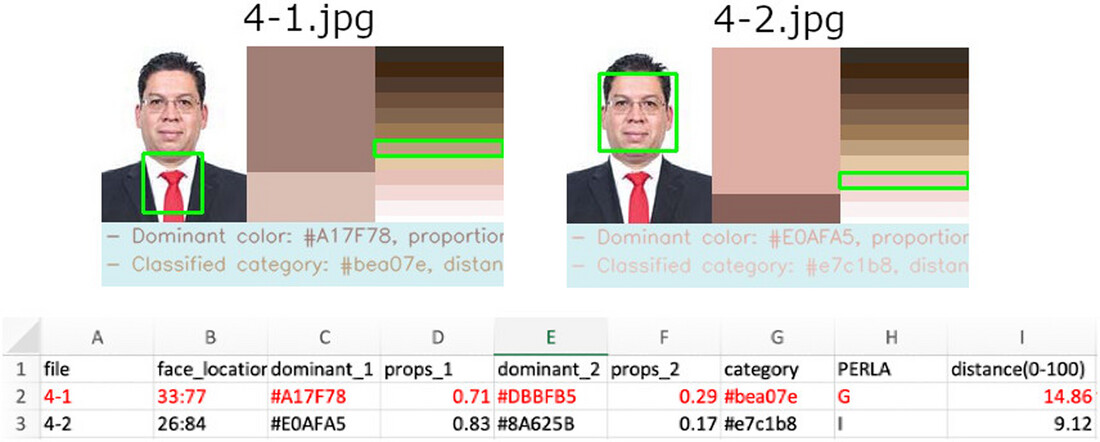
\includegraphics[scale=3]{Template_Latex_TCC-UNIFTEC/_lib/imagens/casco.jpg}

\label{fig:x casco-miss-identification}
\centering{\Fonte{\cite{Classification_Algorithm_for_Skin_Color_CASCo_A_new_tool}.}}
\end{figure}


O processo de identificação de cor de pele é uma das etapas para a identificação de pele, contudo, a detecção de coloração de pele continua sendo um desafio para o processamento de imagem \cite{Human_Skin_Color_Detection_Technique_Using_Different_Color_Models}. Recentemente, com os novos desenvolvimentos em visão computacional, vários trabalhos tentaram classificar a cor da pele a partir de imagens. Apesar de, utilizando imagens, a detecção da cor da pele fica suscetível a influência de vários fatores, como características da câmera, etnia, sombras, iluminação, cores de fundo de movimento \cite{Human_Skin_Detection_Using_Different_Color_Spaces}.
 
Quanto mais tons de cor da pele são utilizados para classificação, mais os tons estão próximos uns dos outros e mudanças de iluminação tornam a cor ainda mais difícil de diferir. Entretanto, no campo da dermatologia e antropometria, a cor da pele é classificada em um nível alto de granularidade, sendo de 6 e 36 tons de pele, respectivamente \cite{Automatic_Skin_Tone_Extraction_for_Visagism_Applications}. Esquemas de classificação mais complexos são altamente subjetivos e apresentam problemas mesmo para os humanos. Um modelo com seis cores é considerado ideal, pois os seis tons combinariam o que podemos distinguir visualmente entre diferentes regiões e raças humanas como cores de pele predominantes \cite{Visagismo}. No entanto, estudos práticos mostram que a classificação natural e não influenciada de cores da pele executadas por humanos conteriam apenas três classes: branco/claro, pardo e preto. Porém, mesmo com três classificações, a classificação é subjetiva.


\section{Extração das características}
De acordo com \cite{rehem2009tecnicas} a extração de características se baseia na extração de informações que compõem a imagem, como textura, bordas, formatos e movimentos. Para isso é necessário realizar uma análise píxel a píxel para comparação, usando alguma métrica de similaridade ou dissimilaridade, podendo haver ou não preocupação com detecção falsa, ou falhas na detecção. Além da possibilidade de marcação de limites para a extração de características, é possível utilizar de suavização de imagem por desfoque para eliminação de ruídos.

Da mesma forma que ocorre na detecção de pele, a detecção de cores é sensível a dispositivos de captura e condições de iluminação, como luminosidade, contraste, transparência, brilho e saturação \cite{Human_Skin_Detection_Using_RGB_HSV_and_YCbCr_Color_Models}. Mesmo com pouca alteração de balanço de branco, na cor da pele há diferentes efeitos em retratos digitais \cite{Skin_Color_Perception_in_Portrait_Image_and_AR_based_Humanoid_Emoji}. O ser humano é bom em identificar cores em diferentes iluminações, o que pode ser definido por consistência de cor \cite{Skin_detection_ashort_tutorial}. Contudo, consistência de cor é relativo à percepção, tornando um desafio para a detecção de pele a representação de cores sem a variação e sensibilidade a iluminação. Por isso, o tom da pele é muitas vezes a combinação de outras características, como textura e recursos de borda. Considerando isso, a detecção de tom de pele para ser otimizada deve considerar a combinação dos fatores mencionados anteriormente em uma faixa de valores ideais, além de considerar as bordas de um rosto, que pode ser obtido a partir da divisão de pixels de uma imagem em pixels individuais e classificando-os em regiões de pele e não pele.\cite{Human_Skin_Detection_Using_RGB_HSV_and_YCbCr_Color_Models}.

\subsection{Thresholding}
 A classificação por \textit{thresholding} é normalmente baseada na propriedade de nível de cinza. Para cada pixel, o mesmo valor limite é aplicado. A classificação de limite binária determina que se o valor do pixel for menor que o limite pré-definido, o limite será definido como 0, sendo marcado por pixel de cor preta, caso contrário, é definido como um valor máximo, marcado como 1. Há também a possibilidade de marcação de limite adaptativo onde se determina o limite para um pixel com base em uma pequena região ao seu redor. A função do OpenCv \textit{threshold}, por exemplo, é usada para aplicar o limite, sendo fornecido diferentes tipos de limite\footnote{https://docs.opencv.org/4.x/d7/d4d/tutorial\_py\_thresholding.html}. A determinação de limite pode auxiliar em momentos em que se uma imagem tiver condições de iluminação diferentes em áreas diferentes, principalmente o \textit{adaptative thresholding}. Assim, obtemos limites diferentes para regiões diferentes da mesma imagem, o que proporciona melhores resultados para imagens com iluminação variável. 

 
\subsection{Detecção e segmentação de pele}
A detecção e segmentação é um processo em que se destaca as regiões relevantes da imagem, segmentando para processamentos posteriores. A maioria dos sistemas de detecção de pele utiliza a cor como principal atributo para construir modelos matemáticos tratáveis e precisos sobre a cor da pele \cite{Deteccao_de_pele_humana_em_imagens_veiculadas_na_web}. Por isso é possível utilizar a posição das cores identificadas como de pele como primeiro passo. 

Uma das formas para identificar cores de pele é pela detecção de pixel, abordagem conhecida como análise quantitativa \cite{Deteccao_de_pele_humana_em_imagens_veiculadas_na_web}. Nesta abordagem os pixels com as mesmas características são contados e agrupados para análise posterior. Assim, um sistema de detecção de pele, que utiliza aprendizado de máquina com base em conjuntos de dados disponíveis, pode usar um classificador treinado para diferenciar um pixel de pele e um sem pele a partir do processo de segmentação, criando intervalo de valores. Em seguida, um conjunto de áreas da imagem é reconhecido como uma imagem de pele, usando sistemas de cores.

 % onde se inclui a validação e satisfação dos dados obtidos. Estimativa de parâmetros sobre a imagem e classificação dos objetos identificados em diferentes categorias.
 
\section{Sistema de Cores}
 Desde a antiguidade, a cor influencia a forma psicológica, fisiológica social e emocional na vida das pessoas \cite{Visagismo}. E a sua percepção é relativa, já que é dependente das relações e interações com outras cores e a tonalidade do fundo \cite{Visagismo}. Por isso, quando se trata de tratamento de imagens, a escolha do sistema de cores é importante.

Os sistemas de cores ou modelos de cores são modelos matemáticos abstratos que representam as informações de cor por meio de diferentes componentes. A escolha do sistema de cores é crítica para a classificação das cores. Cada sistema representa os recursos de cores de maneiras distintas, de forma que as cores sejam mais bem distinguidas e mais adequadas. Os sistemas de cores mais utilizados no processo de reconhecimento de imagem de pele são o RGB, HSV, Lab e YCbCr \cite{Modelo_matematico_para_reducao}, nos quais cada um possui diferentes aplicações em processamento de imagem, computação gráfica, exibição de conteúdo, impressões, entre outros.

No caso da classificação do tom de pele, o problema passa a ser mais difícil. Quanto mais tons são agregados como parâmetro, mais próximos e semelhantes passam a ser as cores, e isso impacta a classificação. Além disso, a rotulagem da cor da pele é muitas vezes considerada subjetiva, mesmo por profissionais treinados \cite{Automatic_Skin_Tone_Extraction_for_Visagism_Applications}.
Por isso a escolha do sistema de cor afeta o desempenho de qualquer algoritmo de detecção de tom de pele, além da sensibilidade às condições de luz \cite{Skin_detection_ashort_tutorial}. Outro desafio se refere a objetos que possuem tons próximos a tons de pele como a madeira, couro, roupas nos tons nude e cabelo. O que pode acarretar detecções com falso positivos quando o ambiente e fundo não são controlados.


\subsection{Modelo RGB}
O sistema de cores RGB (\textit{Red, Green, Blue}) é comumente usado em imagens digitais e se assemelha a codificação de cores do olho humano \cite{Visão_Computacional_Indexação_Automatizada_de_Imagens}. O sistema codifica as cores como uma combinação aditiva de três cores primárias: vermelho (R), verde (G) e azul (B), que representam as frequências baixas, médias e altas, respectivamente, do espectro da luz visível. O espaço de cor formado é um cubo onde nos vértices estão as cores primárias e as secundárias, além da cor preto, para ausência de cores, e o branco, para a presença das 3 cores, conforme a Figura \ref{fig: RGB }. Normalmente, com valores do eixo variando entre 0 a 255 \cite{Cor_Aspectos_relevantes_para_viualização_de_cor}. 

\begin{figure}[h]
\caption{RGB}
\centering

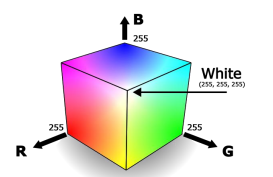
\includegraphics[]{Template_Latex_TCC-UNIFTEC/_lib/imagens/RGB.png}

\label{fig: RGB }
\centering{\Fonte{\cite{}.}}
\end{figure}

Sua principal vantagem é a sua simplicidade. No entanto, o RGB não é perceptivamente uniforme, o que significa que as distâncias no espaço RGB não correspondem linearmente à percepção humana. \cite{Skin_detection_ashort_tutorial}. Além disso, as cores no espectro RGB não separam luminância\footnote{} e crominância\footnote{}, e os componentes R, G e B são altamente correlacionados. A luminância de um determinado pixel RGB é uma combinação linear do R, valores G e B. Portanto, alterar a luminância sobre a pele afeta todos os três componentes. O que conclui que a cor de pele mudará com base na intensidade da iluminação, o que em um tratamento de foto não é o ideal. Apesar dessa limitação, o RGB é extensivamente usado na literatura de detecção de pele devido à sua simplicidade e dependendo do método utilizado pode ter resultados satisfatórios.


 \subsection{Modelo YCbCr}
O modelo YCbCr é uma transformação do espaço RGB \cite{Deteccao_de_pele_humana_em_imagens_veiculadas_na_web}. Neste modelo, as cores são representadas pelo componente \textit{Y}, o qual representa a informação de luminância, e por dois componentes de crominância, \textit{Cb} representa a crominância azul e \textit{Cr} a crominância vermelha, conforme ilustrado na Figura \ref{fig: ycbcr }. Por este motivo podem ter o brilho e a cromaticidade separados. 

\begin{figure}[h]
\caption{}
\centering

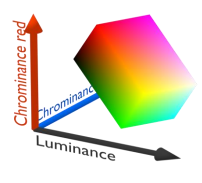
\includegraphics[]{Template_Latex_TCC-UNIFTEC/_lib/imagens/ycbcr.png}

\label{fig: ycbcr }
\centering{\Fonte{\cite{}.}}
\end{figure}

A conversão do espaço RGB para o YCbCr possui vantagens, pois para a visão humana há a sensibilidade maior a luminância. O que possibilita separar e reduzir a quantidade de bits utilizados para a crominância sem perder a qualidade das imagens perante a visão humana. Por conta disso, o YCbCr é um modelo bastante utilizado no contexto de imagens digitais e processamento de vídeo.
 
\subsection{Modelo HSV}
O modelo de espaço de cor HSV é um modelo perceptual, ou seja, o espaço descreve a cor mediante atributos relacionados a percepção da coloração \cite{Deteccao_de_pele_humana_em_imagens_veiculadas_na_web}. É baseado em Matiz-Saturação e é também muito utilizado na área de detecção de pele. Esse modelo é separado em três componentes de tonalidade, tonalidade(H), saturação(S) e brilho(V). O componente H descreve a cor dominante como vermelho, verde, azul, de uma área. O componente S mede a coloração de uma área proporcional ao brilho com variações a cor cinza até as cores totalmente saturadas. Já o componente V referir-se a iluminação, conforme ilustrado na Figura \ref{fig: hsv}.

 \begin{figure}[h]
\caption{}
\centering

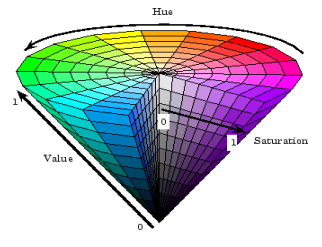
\includegraphics[]{Template_Latex_TCC-UNIFTEC/_lib/imagens/HSV.png}

\label{fig: hsv}
\centering{\Fonte{\cite{}.}}
\end{figure}

 Um dos benefícios deste modelo é que ele permite adicionar a intuitividade e a separação entre tonalidade e saturação, já que o componente V traz a informação de brilho, facilitando a redução de influência de iluminação no tratamento de imagens \cite{Skin_detection_ashort_tutorial}.
 
 \subsection{Modelo CIE-Lab} 
O modelo CIE-lab ou L*a*b é um modelo de cor colométrico definido pela Comitê Internacional de Iluminação (\textit{Commission Internationale d’Eclairage} - CIE). CIE-Lab é um modelo que separa a luminância(L) das outras duas variáveis de crominância (a,b), conforme a Figura \ref{fig: cielab}. Este é um modelo pouco utilizado já que a conversão a partir do RGB é mais cara computacionalmente \cite{Skin_detection_ashort_tutorial} comparado aos outros modelos.

\begin{figure}[h]
\caption{}
\centering

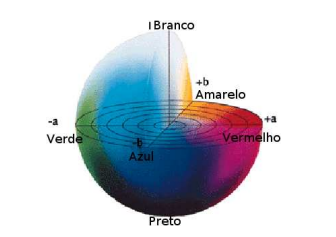
\includegraphics[]{Template_Latex_TCC-UNIFTEC/_lib/imagens/cielab.png}

\label{fig: cielab}
\centering{\Fonte{\cite{}.}}
\end{figure}
 
Segundo o estudo \cite{Automatic_Skin_Tone_Extraction_for_Visagism_Applications},
a precisão da classificação depende de qual sistema de cor é utilizado no processo. Para a comparação, a Tabela \ref{table:Tabela_comparativa_sistemas_de_cores} demonstra a relação de sistema de cor e precisão para detecção de tom de pele.

% Please add the following required packages to your document preamble:
% \usepackage{graphicx}
\begin{table}[]
\centering
\caption{Tabela Comparativa Sistemas de Cor}
\label{table:Tabela_comparativa_sistemas_de_cores}\textbf{}
\begin{tabular}{lll}
\hline
  & Sistemas de Cor                   & Precisão \\ \hline
1 & R, G, B                           & 74.65\%  \\
2 & H, S, V                           & 83.30\%  \\
3 & L, a, b                           & 72.46\%  \\
4 & Y, Cr, Cb                         & 83.30\%  \\
5 & L, a, b, H, S, V                  & 85.18\%  \\
6 & L, a, b, Grayscale                & 84.19\%  \\
7 & L, a, b, H, S, R, G, B, Y, Cr, Cb & 86.67\%  \\ \hline
\end{tabular}%
\centering{\Fonte{Autor}}
\end{table}

Frente a diversificada forma de descrever uma tonalidade de pele usando diferentes espaços de cor, neste estudo foram destacados os espaços de cor RGB, YCbCr e HSV, amplamente utilizados em equipamentos de captura, por exemplo, câmeras fotográficas e filmadoras digitais. 

O modelo de cor de pele é produzido com base em rostos
individuais. No entanto, a literatura ainda carece de evidências sobre
qual escala é adequada para ser usada como método de detecção
dinâmica da cor da pele.

\subsection{Processamento de alto nível}
%onde se inclui a validação e satisfação dos dados obtidos. Estimativa de parâmetros sobre a imagem e classificação dos objetos identificados em diferentes categorias. %

\section{Classificação em Imagens Digitais}
A classificação envolve rotular os pixels de forma que cada um se enquadre em uma classe. Para isso há técnicas supervisionadas e não supervisionadas. Nesse trabalho será abordado a classificação não supervisionada como o \textit{K-means}.

\section{Classificação Não-supervisionada}
As técnicas não-supervisionadas classificam cada pixel de uma imagem em um determinado classe sem o número prévio de classes existentes, agrupando os dados inseridos.

\subsection{Algoritmo K-means} %nao supervisionado
Impulsionado não apenas pela indústria cosmética, mas também pela ciência da visão computacional, um esforço significativo foi feito para coletar os verdadeiros valores da cor da pele, principalmente com foco no rosto. Para a identificação do que é pele e não pele em uma imagem se muito utilizado as técnicas de detecção de pele classificadas como técnicas baseadas em pixels ou técnicas baseadas em regiões. Nessa detecção é classificado como pixel de pele ou não pele individualmente, dependendo de certas condições, como cores e regiões consideradas regiões de pele. Inicialmente a região da pele cresce adicionando mais pixels com base nas propriedades de seus vizinhos.

\begin{figure}[h]
\caption{}
\centering

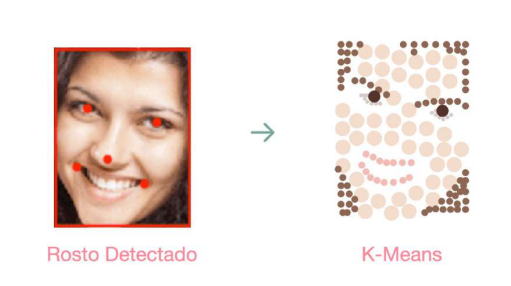
\includegraphics[]{Template_Latex_TCC-UNIFTEC/_lib/imagens/kmeans.png}

\label{fig: kmeans }
\centering{\Fonte{\cite{Uso_visao_computacional_para_reconher_marcas_maquiagem}}}
\end{figure}


\subsection{Validação}
Distância Euclidiana 
Distancia delta e2000

uso de biblioteca scikit-image

\label{cap:fundamentacao-teorica}
    \chapter{Metodologia}
\label{cap:metodologia}

\subsection{Revisão Sistemática da Literatura}
 Nesse capítulo é apresentada a metodologia de Revisão Sistemática da Literatura utilizada para o rastreio de trabalhos relacionados. Este, o qual, possui o intuito de pesquisar artigos e trabalhos relacionados e aprofundar os conhecimentos sobre o tema proposto, com objetivo de entender as abordagens utilizadas no meio científico e os desafios a fim de aperfeiçoar o desenvolvimento deste projeto. Conforme essa metodologia, foram seguidas as seguintes etapas:
 
Na primeira etapa, buscou-se por artigos e trabalhos relacionados nas bases digitais de pesquisa Google Acadêmico\footnote{https://scholar.google.com/}, IEEE Xplore\footnote{https://ieeexplore.ieee.org/Xplore/home.jsp} e Researchgate\footnote{https://www.researchgate.net/}. Nelas foram aplicadas sentenças de busca por palavras-chave que trouxessem trabalhos relacionados ao tema proposto. 

Organizado por relevância acadêmica e por pesquisa avançada, filtrando-se as pesquisas com as palavras-chave alcançou-se a seguinte expressão:

\begin{center}
\centering
\textbf{(("All Metadata":skin color) OR ("All Metadata":skin undertone) OR ("All Metadata":skin tone) OR ("All Metadata":artificial inteligence) OR ("All Metadata":neural network) OR ("All Metadata":diversity) OR ("All Metadata": computer vision) OR ("All Metadata":inclusion) OR ("All Metadata":beauty industry) OR ("All Metadata":cosmetics industry) OR ("All Metadata":skin color detection) NOT ("All Metadata":texture) NOT ("All Metadata":lesion) NOT ("All Metadata":medical) NOT ("All Metadata":cancer) NOT ("All Metadata":melanome))}
\end{center}


Na segunda etapa, foi realizado a triagem dos artigos anteriormente encontrados onde se buscou por artigos publicados entre os anos de 2018 e 2023. Em seguida, na terceira etapa foi realizada a leitura utilizando os títulos e resumos como critério de seleção. Nessa etapa foi visto que a maioria dos artigos selecionados anteriormente tinham como foco principal identificar pele em imagens e vídeos sendo a identificação da cor de pele somente uma etapa do processo e sem classificação das mesmas. Na quarta etapa foi feito a leitura completa dos artigos e buscou-se verificar a adequabilidade dos artigos selecionados. 

Como critério de análise dos artigos de inclusão levou-se em conta a abordagem dos estudos relacionados ao desenvolvimento de cosméticos e abordagens gerais utilizando \textit{Machine Learning}. Como critério de exclusão optou-se por não considerar artigos relacionados a problemas de saúde na pele como câncer de pele e feridas, apesar de ser um tópico bastante estudado utilizando técnica de inteligência artificial para identificação coloração de pele, segmentação e classificação. Como já é conhecido que a maioria das pesquisas realizadas sobre a análise da cor da pele é focado na detecção de pele\cite{A_survey_of_skin-color_modeling_and_detection_methods}. Como resultado foram encontrados no total 69 artigos, analisados os resumos passaram-se a 35 artigos e após as quatro etapas do RSL restaram somente 4 trabalhos relacionados.

A metodologia deste estudo consistiu em quatro
etapas principais, ou seja, detecção de face, amostragem de pele por imagem, extração de pixel de pele e classificação de pixel de pele. Ao
longo deste artigo, nosso método é uma classificação baseada em
pixels, onde os pixels são a principal característica



Detecção de cor de pele é um processo para encontrar pixels com tons de pele em regiões definidas a partir de uma imagem. 

\subsection{Materiais e Métodos}
Para os experimentos abordados no desenvolvimento foi utilizado a linguagem Python\footnote{https://www.python.org/doc/essays/blurb/}. A escolha da linguagem se deu pela facilidade de uso e pela quantidade de estudos na área de \textit{Machine Learning} que utilizam a mesma.

LEITURA DE DATASET STILL UNDEFINED.ATUALMENTE UTILIZANDO BIBLIOTECA IMUTILS PARA LER UMA UNICA IMAGEM POR VEZ.





As funções que implementam as validações de modelo como o cálculo de precisão, acurácia, margem de erro foram construídos utilizando a biblioteca Scikit-learn\footnote{https://scikit-learn.org/stable/about.html} . 




(deve aparecer os objetivos)

(como validar?)
	\chapter{Trabalhos Relacionados}
\label{cap:trabalhos-relacionados}
Este capítulo apresenta trabalhos que possuem relação com o tema proposto, resultantes do processo da Revisão Sistemática da Literatura. Neste capítulo o objetivo é apresentar o resumo dos 4 artigos selecionados e esclarecer qual o objetivo das pesquisas, os métodos utilizados e seus resultados.

\section{Facial skin colour classification using machine learning and hyperspectral imaging data} 

Segundo o estudo \cite{Facial_skin_colour_classification_using_machine_learning_and_hyperspectral_imaging_data}, a indústria da beleza enfrenta a falta de métodos precisos para classificar automaticamente a cor da pele, pois utiliza rótulos de granularidade alta, como a escala Pantone, a qual é utilizada na \textit{Skin Tone Guide} e abrange até 110 tipos de cor de pele facial. Neste contexto, o estudo examinou tecnologias projetadas para coletar dados de cores de pele, bem como métodos para classificar com precisão os tipos de cores de pele usando a escala Pantone como referência.
 
% Segundo o estudo \cite{Facial_skin_colour_classification_using_machine_learning_and_hyperspectral_imaging_data}, a indústria da beleza carece de métodos precisos para classificar automaticamente a cor da pele porque utiliza de rótulos de alta granularidade, como a escala Pantone utilizado na \textit{Skin Tone Guide} que detém até 110 tipos de cor de pele facial. Com isso, nesse estudo foi examinado tecnologias projetadas para coletar dados de cores de pele faciais e métodos para classificar com precisão os tipos de cores de pele faciais usando a escala Pantone como base.

A classificação automática da cor da pele do rosto foi realizada com base em imagens hiperespectrais e aprendizado de máquina.  A imagem hiperespectral, conhecida como imagem espectral ou química, é uma tecnologia de medição não invasiva usada para coleta de dados que já é utilizada para medir a saúde da pele. E, para auxiliar nisso, foi avaliado seis métodos de aprendizado de máquina aplicados a esses dados e comparados e descobriu-se que cada um tinha uma vantagem na categorização de um subconjunto de tipos de cores, além disso, foi abordado a classificação para a cromaticidade e brilho para alcançar a precisão mínima de 90\% de precisão.

A metodologia utilizada é referenciada como aprendizado de máquina \textit{offline} supervisionado, já que o tipo de cor correto é conhecido e baseado no Guia da Pantone, e os dados foram coletados antes do início do aprendizado. Contudo, o experimento teve desafios, principalmente ao  coletar \textit{big data} sobre a cor da pele do rosto por meio de imagens hiperespectrais para a classificação da cor da pele facial.  Primeiro desafio se referiu à coleta de dados multidimensionais nos diferentes tipos de cores de pele e à alta granularidade dos tipos de tom da pele. O segundo, ao classificar o tipo de cor com precisão, considerando que imagens espectrais são influenciadas por fatores ambientais. E, terceiro, ao escolher o melhor método de classificação projetados para classificar os tipos de cores faciais com base nos dados de imagens hiperespectrais de modo que alcancem precisão mínima esperada.

O experimento baseou-se na geração de imagens hiperespectrais em laboratório utilizando um gerador da marca Photon para registrar imagens de 108 tipos de cores do Guia Pantone de Tons de Pele, onde cada cor era representado por um cartão. A partir disso, os cartões eram iluminados com altura, distância, temperatura e umidade padrões, assim a luz incidida no cartão era refletida e capturada pelo equipamento. Cada cartão foi medido 20 vezes para minimizar a perda de dados. Apesar das medições repetidas, foi necessário analise e classificação  dos dados brutos para identificar possíveis anomalias nas medições, considerando a média das intensidades luminosas e as distâncias euclidianas entre a média de cada medição. Tendo como resultado das 2160 medições apenas 1725 medições válidas. Assim, para resolver a classificação dos tipos de cor foi explorado métodos de aprendizagem automática.

No estudo, foram utilizados oito classificadores com seis métodos de classificação diferentes em que foram comparados as suas taxas de precisão, sendo eles regressão logística, KNN, SVM com kernel linear, SVM com kernel radical, SVM com kernel polinomial, árvore de decisão, reforço adaptativo e floresta aleatória. Como pode ser visto na Figura \ref{fig:x classificacao} o método de floresta aleatória teve a precisão mais elevada de 88\%, seguida da SVM com função de kernel radical, reforço adaptativo e KNN acima de 50\%. Contudo, ao se comparar a diferença de precisão na classificação por tipos de cor, o método de regressão logística possuía a menor precisão para todos os tipos de cor entre os classificadores. E, os outros classificadores, exceto a regressão logística, obtiveram uma vantagem de precisão em diferentes tons de pele. Isso resultou na necessidade de integrar os métodos para melhorar a desempenho da precisão dos métodos escolhidos para a classificação de tipo de cor de pele facial.

\begin{figure}[h]
\centering
\caption{Precisão de classificação entre os oito classificadores}
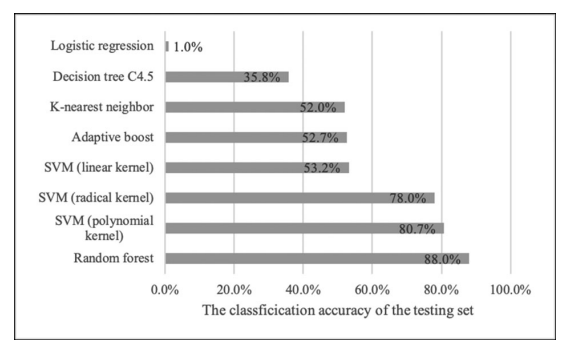
\includegraphics{Template_Latex_TCC-UNIFTEC/_lib/imagens/resultados_facial_skin.png}

\label{fig:x classificacao}
\centering{\Fonte{\cite{Facial_skin_colour_classification_using_machine_learning_and_hyperspectral_imaging_data}}}
\end{figure}

Para explorar os pontos fortes dos classificadores, foi proposto um classificador integrado de dois estágios que empilha seus resultados para produzir uma nova previsão e validação cruzada por 10 vezes. Na primeira etapa, foi utilizado sete classificadores usando um conjunto de treinamento e, em seguida, aplicado a outro conjunto de treinamento. As saídas dos classificadores formam uma nova entrada independente de sete dimensões atributos.  Na segunda etapa, foi utilizado o conjunto de treinamento para construir uma floresta aleatória empilhada classificador. A partir disso, a segunda abordagem proposta alcançou 89,4\% de precisão no conjunto de teste. Esta foi uma ligeira melhoria em relação à precisão de 88,0\% do classificador básico de floresta aleatória, mas ainda ficou aquém da exigência prática de 90\% de precisão.

Ao analisar as características dos dados coletados descobriu-se que a cromaticidade e o brilho da pele podem ser classificados separadamente, e fornecem informações relevantes. Por isso, para melhorar mais a precisão  dos dados, eles foram classificados conforme o tipo de cor. Cada tipo de cor de cartão foi dividido em subtipos de cromaticidade e brilho. A cromaticidade mede a qualidade da cor, e o brilho mede a intensidade da luz e segundo o Guia Pantone de Tom de pele há 10 classes de cromaticidade e 15 classes de brilho.

A classificação de subtipos por cromaticidade permitiram refinar os classificadores melhorando a precisão, já que houve diferenças discrepantes entre elas, sendo que algumas que exibiram menor intensidade e outras maiores intensidade em todos os espectros. Isso resultou no aumento da precisão no método floresta aleatória para 95,9\% o que pode ser visto na Tabela \ref{table:Tabela_comparativa_entre_os_métodos_e_precisões}.

Já a classificação de subtipos por brilho considerou 15 espectros de brilho. Os dados mostraram que o nível mais altos sofreram mais distinção que os outros, contudo eles acabaram criando cluster entre os níveis. Contudo, a classificação do subtipo de brilho foi significativamente menos precisa. Assim, os subtipos de brilho foram mais difíceis de distinguir um do outros em comparação com a cromaticidade.


\begin{table}[]
\centering
\caption{Tabela comparativa entre os métodos e precisões}
\label{table:Tabela_comparativa_entre_os_métodos_e_precisões}\textbf{}
\resizebox{\columnwidth}{!}{%
\begin{tabular}{lllll}
\hline
Algoritmo classificador & Precisão & Precisão por nível de cromaticidade & Precisão por nível de brilho &  \\ \hline
Regressão Logística     & 1.0\%    & -                                   & -                            &  \\
Árvore de decisão       & 35.8\%   & 29.4\%                              & 20.6\%                       &  \\
K-nearest neighbor      & 52.0\%   & 69.7\%                              & 59.6\%                       &  \\ 
Impulso Adaptativo      & 52.7\%   & 70.6\%                              & -                            &  \\
SVM (kernel linear)     & 53.2\%   & 81.7\%                              & 61.9\%                       &  \\
SVM (kernel radical)    & 78.0\%   & 79.8\%                              & 56.4\%                       &  \\
SVM (kernel polinomial) & 80.7\%   & 85.3\%                              & 53.7\%                       &  \\
Floresta aleatória      & 88.0\%   & 95.9\%                              & 83.9\%                       & \\ \hline
\end{tabular}%
}
\centering{\Fonte{Autor}}
\end{table}


Um exame detalhado dos resultados revelou que quanto maior classes de brilho foram classificadas com maior precisão do que as classes inferiores. Além disso, cada classificador exibiu algumas vantagens porque cada um teve um desempenho melhor do que outros para determinados tipos de brilho. As informações sobre a classificação do subtipo de brilho foram utilizadas para melhorar a precisão por meio do método de dois estágios classificador integrado semelhantemente à utilização das informações de cromaticidade. No final foi construído um classificador integrado de dois estágios com empilhamento de modo que as saídas de classificação do subtipo de brilho dos seis classificadores foram adicionadas como o terceiro conjunto de novas entradas para a floresta aleatória de empilhamento. Finalmente, o empilhamento floresta aleatória tinha 20 atributos como entradas, dos quais sete eram tipos de cores, sete eram subtipos de cromaticidade e os últimos seis eram subtipos de brilho.
Isso possibilitou que o estudo alcançasse 95.9\% de precisão, porém juntando as metodologias a precisão da classificação do tipo de cor alcançada ficou em 90,4\%. Resultado que ficou acima do objetivo esperado e conclui que este classificador pode ser usado pela indústria da beleza para avaliar o efeito dos produtos para a pele na cor da pele do rosto.


\section{Human Skin Tone Detection}

Neste artigo \cite{Human_Skin_Tone_Detection}, os autores apresentam a proposta de uma aplicação completa que detecta, a partir de uma imagem, a cor de pele, classificando o tom de pele analisado em três tons básicos: claro, médio e escuro. Como proposta, o trabalho aborda o desenvolvimento de um aplicativo que recebe imagens e utiliza \textit{Machine Learning} para detectar o tom de pele e a partir da análise retorna a classificação de tonalidade da imagem de um rosto. Além de desenvolver a aplicação, o objetivo dos autores é desenvolver um método eficiente e preciso para detectar o tom da pele humana em imagens. Como aplicação foi proposto um sistema que seja executável em qualquer sistema operacional disponível e navegadores empregando no \textit{front-end} HTML, CSS, Bootstrap4 e Python com banco de dados MySQL.

A metodologia proposta envolve o reconhecimento facial da imagem, a identificação das características faciais, remoção de pixels escuros com segmentação de pele, a extração e  a classificação dos pixels nas três categorias de tonalidades.E como chave para a construção da aplicação amigável ao usuário, os requisitos para isso se resumem em carrega o arquivo de imagem, identificar o tom de pele e fornecer a cor do tom. Para demonstrar melhor o fluxo de trabalho do sistema, a Figura \ref{fig:x human_detection} ilustra o fluxograma da metodologia utilizada no processamento de imagem e o resultado esperado para o tom claro e escuro.

\begin{figure}[h]
\centering
\caption{Fluxograma de metodologia da aplicação}
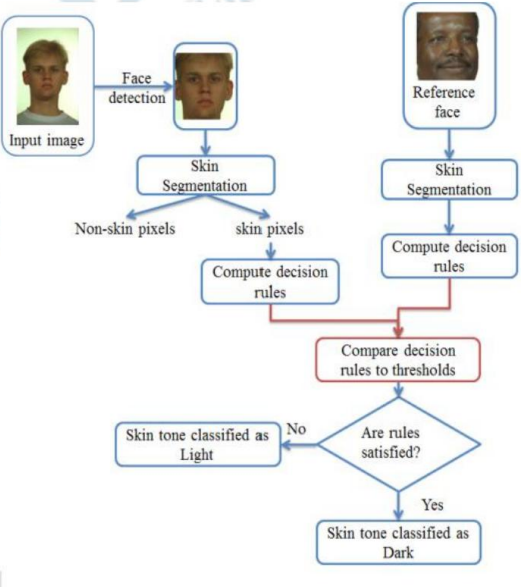
\includegraphics[]{Template_Latex_TCC-UNIFTEC/_lib/imagens/human_skin_detection.png}

\label{fig:x human_detection}
\centering{\Fonte{\cite{Human_Skin_Tone_Detection}.}}
\end{figure}

Para a etapa de reconhecimento facial, é necessário identificar a face na imagem carregada e segmentar a imagem para separar regiões com a presença e a não presença de pele. Para isto, foi substituído o modelo Gaussiano por não apresentar precisão mínima, apesar de sua simplicidade, e passou-se ao modelo elíptico. O modelo de limite elíptico utiliza a técnica de compensação de iluminação para corrigir o viés de cor e converter os componentes do modelo RGB para o espaço de cor YCbCr. Em seguida, os pixels de tom de pele são detectados por meio de um modelo de pele elíptico no novo espaço de cor. Os pixels detectados são segmentados iterativamente com base na variação de cor local, agrupados em pixels de coloração semelhante da região analisada, no caso, o rosto, considerando o arranjo espacial desses componentes e a semelhança de suas cores. Assim, o módulo de detecção de características faciais rejeita regiões candidatas de rosto que não contenham nenhuma característica facial, como olhos, boca e contorno facial. Após o processamento da imagem, as características são extraídas do conjunto de imagens e as cores são comparadas com as categorias propostas a partir de uma referência. Uma vez que a extração do tom de pele é realizada pelo algoritmo de aprendizado de máquina, os dados obtidos são enviados de volta ao servidor, são armazenados no banco de dados e, por fim, o resultado é exibido na página de \textit{front-end} para o usuário.

Como próximos passos, foi proposto primorar o sistema de reconhecimento de variação de cor facial adicionando pré-modelos mais detalhados e precisos e automatizar o processo para apresentar os resultados em um aplicativo web ou \textit{desktop}. Assim, como permitir o processamento em tempo real e adicionar o reconhecimento de outras variações de tons de pele, além dos tons comuns básicos. 

\section{Automatic Skin Tone Extraction for Visagism Applications}
 O estudo em \cite{Automatic_Skin_Tone_Extraction_for_Visagism_Applications}, propôs um sistema de classificação de pele em três tons, pele clara, média e escura para auxiliar na seleção de óculos, utilizando dois métodos.
 
O primeiro método utiliza as etapas convencionais do aprendizado de máquina com seleção da região de interesse, extração de características e classificação. Combinando e organizando vários espaços de cores em histogramas de manchas de pele e reduzindo o espaço de recursos resultante, de modo que apenas os recursos com alto poder discriminativo sejam mantidos para votação. Foi usado um classificador SVM treinado para rotular as cores de pele.

\begin{figure}[h]
\caption{Fluxograma de classificação por SVM }
\centering

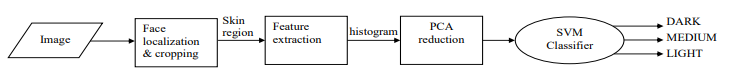
\includegraphics[]{Template_Latex_TCC-UNIFTEC/_lib/imagens/FluxogramaVisagismo.png}

\label{fig:x fluxogama_svm}
\centering{\Fonte{\cite{Automatic_Skin_Tone_Extraction_for_Visagism_Applications}.}}
\end{figure}

Primeira etapa do método é a identificação do rosto a partir da imagem e para isso foi utilizado o algoritmo Viola-Jones. Para evitar as partes irrelevantes como olhos, lábios e cabelos, foram cortadas as regiões de interesse (ROI) como abaixo dos olhos e acima do centro da face para melhor classificar o tom de pele. Em seguida, foi feito o vetor de características composto por 13 histogramas (3 espaços de cores e tons de cinza) baseado nos resultado dos quatro sistemas de cores, sendo eles RGB, HSV, Lab e YCrCb. A partir disso os dados alimentar o SVM para obter o tom de pele da região dominante no ROI.

O segundo método utiliza \textit{Deep Learning} com os estágios clássicos de aprendizado de máquina substituídos
pela rede neural convolucional (CNN) para extrair automaticamente recursos cromáticos de conjuntos aumentados de imagens faciais. Ambos os algoritmos foram treinados e testados em conjuntos de dados disponíveis publicamente. 

Para a CNN foi utilizada a rede VGG-19 que foi treinada previamente para reconhecimento de gênero a partir de imagens faciais com uma base de 200.000 imagens. Para detectar tom de pele, as duas ultimas camadas da CNN foram removidas para a parte restante ser usava como um extrator de recursos. Por fim, um classificador linear foi treinado para o problema de classificação de tom de pele utilizando as características previamente aprendidas pela CNN.

Para as etapas de treinamento e teste para ambos os métodos foram utilizadas imagens faciais da Internet e de diferentes bancos de dados disponíveis publicamente como Caltech, Chicago Face, Minear-Park e banco de dados de faces brasileiras por Thomaz e Giraldi. Cada banco possui diferentes características como controle ou não de ambiente e iluminação. Além de usar imagens faciais de celebridades selecionadas.

Para determinar o tom de pele real, cada amostra de imagem foi anotada independentemente por três pessoas
diferentes e o tom definido pela fusão dos resultados das anotações independentes. Primeiramente, os anotadores tiveram um treinamento com um especialista visagista que os instruiu com as regras que dois seguem no processo de anotação. Durante o treinamento, eles também anotaram com o visagista um subconjunto das imagens e discutiram como lidar com casos, limite e incertezas. Após mesclar os resultados de rotulagem humana, observaram que a maioria das
inconsistências de anotação apareceram entre os tons de pele médios e escuros.

Para melhorar a precisão foram utilizadas técnicas de aumento de contraste e aumento de brilho. O que tornou o algoritmo de aprendizado mais robusto para condições de iluminação. Com isso, o método SVM atingiu a precisão de 86,67\%, enquanto a abordagem CNN obteve uma precisão de 91,29\%. Contudo, foi possível apontar que no método CNN houve mais classificações errôneas entre cores médias claras e médias escuras, o parecido com a classificação conduzida por humanos anteriormente ao longo do estudo. Já na SVM não houve confusões entre cores escura e clara.

\section{Classification Algorithm for Skin Color (CASCo): Anew tool to measure skin color in social science research}
No artigo \cite{Classification_Algorithm_for_Skin_Color_CASCo_A_new_tool} os autores apresentam um algoritmo de classificação para cor de pele, chamado CASCo (\textit{Classification Algorithm for Skin Color}),  que permite identificar e classificar tons de forma objetiva, automática, acessível e personalizável, sem distorções de viés e preconceito racial. A metodologia proposta envolve revisar métodos tradicionais para a medição de tom de pele e observar suas deficiências e a partir disso construir uma ferramenta. Como resultado obteve-se o CASCo, uma biblioteca desenvolvida na linguagem Python que detecta o rosto, segmenta a pele e utiliza k-means para determinar a categoria de tom de pele de imagens.  

Para a detecção de tom de pele a biblioteca realiza a partir de fotos a detecção de face utilizando o sistema HSV para mapear as cores do rosto. O sistema HSV foi escolhido, pois ele é um sistema alinhado à percepção visual que os humanos possuem com relação às características das cores. 
O segundo passo extrai áreas que não contém pele utilizando \textit{threshold} do modelo HSV para restringir, no filtro da função de\textit{ blur} de Gaussian, apenas pele, retirando olhos, cabelos e dentes. Em seguida é utilizado o k-means para identificar duas cores como dominantes.
Como consequência, para categorizar as cores dominantes, é utilizada uma paleta como referência e calculada qual a cor detectada é mais próxima ao peso mínimo Delta E(CIE 2000), ou seja, qual a menor distância delta entre a paleta utilizada e o delta.
A paleta de referência padrão é a paleta PERLA. PERLA é uma paleta que contem 11 tons de pele como referência desenvolvida na Universidade de Princeton visando ajudar estudos de tons de pele na América Latina e já vem sendo utilizada na pesquisa social.Contudo, a biblioteca CASCo aspira ser configurável e a paleta a ser utilizada pode ser facilmente alterada.
Após a implementação, o CASCo tem como resultado a criação de um arquivo de relatório que contém nove colunas com as informações coletadas, sendo elas a imagem avaliada, a localização da face encontrada, a primeira cor dominante identificada e a segunda e as suas proporções de presença da cor da na área facial identificada, a cor PERLA identificada e a distância entre a cor dominante e a cor classificada calculada de 0 a 100. Além disso, é obtido através da modalidade de \textit{debug} a foto utilizada com o resultado da identificação facial e ao lado direito a paleta de cores dominantes e ao lado dela a paleta usada para a classificação com a cor classificada marcada. Abaixo é impresso o valor em hexadecimal da cor dominante e sua proporção e o hexadecimal da categoria da cor classificada e o valor resultante de acurácia. Como pode ser visto na Figura \ref{fig:x resultado_CASCo}.


\begin{figure}[h!]
\caption{Exemplo de resultados obtidos pelo processamento usando CASCo}
\centering

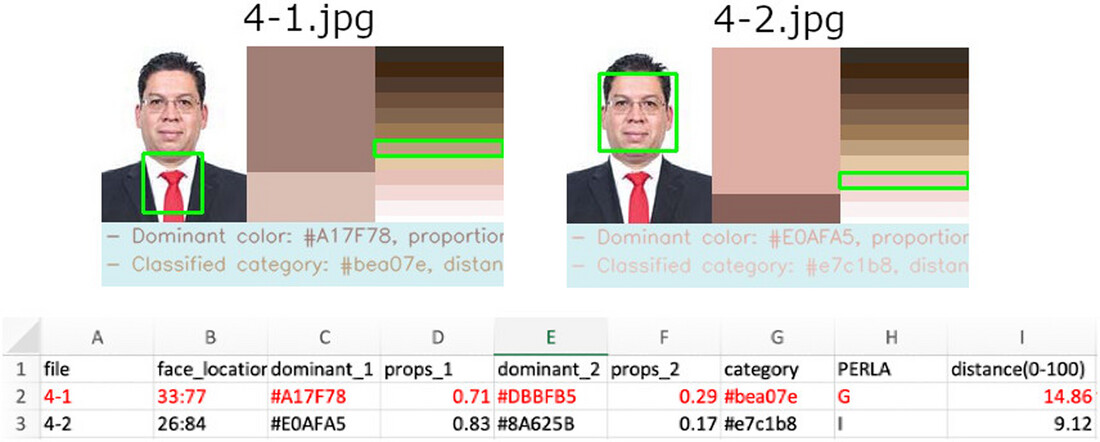
\includegraphics[scale=2]{Template_Latex_TCC-UNIFTEC/_lib/imagens/casco.jpg}

\label{fig:x resultado_CASCo}
\centering{\Fonte{\cite{Classification_Algorithm_for_Skin_Color_CASCo_A_new_tool}.}}
\end{figure}

Na modalidade de \textit{debug} as imagens processadas possuem seus resultados gerados anexados na pasta para verificação dos resultados, \textit{logs} gerados e a planilha \textit{result.csv} com o resumo de cada imagem.

Como fatores limitadores foram citados o próprio uso de imagens para a detecção, principalmente utilizando a pele facial que podem ter por natureza implicações relacionadas a problemas de capturamento e influência de iluminação nos tons de pele, apesar disso por ser uma alternativa barata comparada ao uso de espectrômetros isso seria facilmente burlado utilizando \textit{datasets} prontos reduzindo o esforço na coleta de imagens em novas pesquisas. Ademais, a CASCo possui limitações quanto a identificação caso a pessoa esteja usando maquiagem, por influenciar na correta amostra de pele e causar efeito de esbranquecimento nas peles.

Em suma, a CASCo é uma ferramenta que tem em vista democratizar a pesquisa relacionadas ao tom de pele, facilitando a viabilidade, replicabilidade e objetividade da medição de tons de pele. Apesar das limitações, por ser uma ferramenta customizável é possível introduzir novas paletas de classificação, novos clusters, quantidades de cores dominantes, etc. Também é uma ferramenta que pode processar rapidamente grandes \textit{datasets} de imagens e sem intervenção humana, além de não necessitar de aparelhos caros para medição como espectrômetros para seu funcionamento e ser disponibilizada para uso gratuitamente. Tudo é customizável, bastas os pesquisadores terem as cores hexadecimais ou as cores RGB para utilizar a biblioteca.



\section{Considerações sobre os trabalhos relacionados}

Recentemente, foi possível notar número limitado de trabalhos selecionados na área de identificação de tonalidade de pele, sobretudo pelo fato de a identificação de tom de pele não ser objeto final de muitos artigos, mas sim um dos processos para o reconhecimento facial bem-sucedido. 

Os artigos selecionados procuram identificar tonalidades de pele que não estão concentradas em regiões específicas ou em raças e etnias específicas. Contudo, a seleção se justifica porque a maioria utiliza a área facial para a identificação de tons de pele. Entre eles há escolha de faixas de cores de classificação diferentes, como a utilização do Guia Pantone de Tom de Pele, utilizado pela indústria, a paleta PERLA, criada com base no autorreconhecimento de raça e etnia na América Latina e a classificação classifica do visagismo como de pele clara, média e escura.

Apenas dois trabalhos utilizavam paletas de classificação em comum, contudo entende-se que entre os trabalhos relacionados dificilmente uma paleta irá abordar todos os tons de pele possíveis. Assim como, quanto mais cores forem colocadas para a classificação, mais erros de classificações entre tons parecidos podem ocorrer, como visto no primeiro artigo \cite{Facial_skin_colour_classification_using_machine_learning_and_hyperspectral_imaging_data}. Além disso, principalmente, ao usar humanos no estudo para validar classificações, pode desenrolar influência de viés históricos, étnicos e raciais. Ou seja, mesmo em uma paleta de três tons, uma pessoa em diferentes lugares pode ser classificada por pessoas em diferentes tonalidades, ao ser um tópico também subjetivo.

Com relação ao uso de sistema de cores, os mais usados foram os sistemas YCbCr e HSV, por serem modelos amplamente comuns na detecção de pele e que apresentam melhor resultado comparados aos outros modelos conhecidos. Quanto aos algoritmos de \textit{machine learning} e ferramentas, notou-se maior uso do algoritmo de Viola-Jones, principalmente por ser usadas fotos de rostos em três estudos, SVM e K-means. Além disso, dois dos trabalhos apresentaram valores de precisão superiores a 90\%.

A partir destas constatações, considerou-se que apesar de diferentes ferramentas, os desafios eram equivalentes, sendo possível resumir quais os pilares fundamentais para a implementação do trabalho. Sendo eles, coletar diferentes imagens de pele, tratar imagens considerando problema relacionados a iluminação, escolher sistemas de cores adequados para conversão das imagens e excluir e separar de regiões de pele e não pele nas imagens.



	\chapter{Desenvolvimento}
\label{cap:desenvolvimento}
Este capítulo apresenta o desenvolvimento do sistema responsável pelo processamento de imagens, identificação dos indivíduos e seus tons de pele, detalhando o que cada parte do processo faz e quais parâmetros podem ser alterados para obter-se outros resultados. O processo ocorre em três etapas
distintas. Em um primeiro momento as imagens são inseridas, em seguida é feita a identificação e, finalmente, a classificação.

\begin{figure}[h]
\centering
\caption{Diagrama de desenvolvimento}
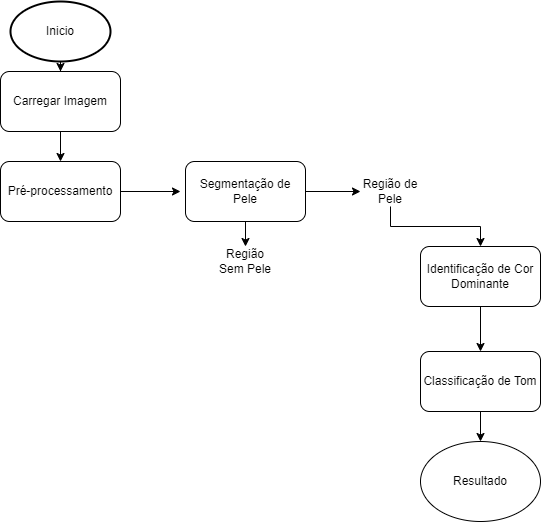
\includegraphics[scale=0.65]{Template_Latex_TCC-UNIFTEC/_lib/imagens/fluxogramaDesenvolvimento.png}

\label{fig: fluxograma_desenvolvimento}
\centering{\Fonte{Autor}}
\end{figure}

A Figura \ref{fig: fluxograma_desenvolvimento} ilustra o processo conceitual básico do sistema proposto para a solução desenvolvida. Para o funcionamento o sistema requer a entrada de uma imagem. A imagem é modificada e convertida para iniciar o pré-processamento. No pré-processamento é executada a identificação da face e regiões a serem excluídas. Em seguida, ocorre a segmentação de pele onde a região de pele e não-pele é separada. Apenas os pixels interpretados como pele são analisados para a identificação de cor dominante e, por fim, a classificação do tom  e saída do resultado com a cor e classificação conforme os tons da paleta de Monk.

Para o desenvolvimento de um sistema para detecção de tom de pele é possível escolher mais de uma região corporal para ser analisada. Contudo, com o objetivo do trabalho mencionado no \ref{cap:introducao}, optou-se pela detecção de face com a pessoa posicionada de frente para a câmera. 

\section{Manipulação de Imagens}
Para a implementação do processo de identificação de tom de pele, foi preciso executar manipulações nas imagens para a realização das etapas de pré-processamento e de resultado visual. Para isso, utilizou-se a biblioteca OpenCV\footnote{https://opencv.org/}. Biblioteca que possui métodos prontos para a manipulação, conversão de imagem e identificação de faces. 

Para o início do processo é preciso a inserção de uma imagem. Para ler as imagens foi utilizado a biblioteca OpenCv com a função imread(). A função imread()\footnote{https://docs.opencv.org/4.x/d4/da8/group\_\_imgcodecs.html\#ga288b8b3da0892bd651fce07b3bbd3a56} carrega uma imagem do arquivo especificado e retorna uma matrix. Além de, ao longo do desenvolvimento foi adicionada a possibilidade de ler imagens utilizando a URL da imagem como entrada com a biblioteca Imutils ao utilizar a função  url\_to\_image() \footnote{https://github.com/PyImageSearch/imutils} e ler uma ou mais imagens a partir de pastas com a função list\_images(). A função url\_to\_image() aceita apenas a URL da imagem. A imagem é baixada e convertida para um array NumPy no formato OpenCV realizando o \textit{download} na memória. A função do list\_images() do módulo paths do Imutils é uma função para localizar imagens recursivamente com base em um diretório raiz. Com isso, foi possível testar uma ou mais imagens por vez na fase de teste relatado no Capítulo \ref{cap:experimentos-resultados}. As três funções permite manipulação de tamanho de imagem, além de permitirem a utilização de vários extensões de arquivo como JPEGs, PNGs, TIFFs e entre outros.

Para a validação da identificação de pele foram utilizadas imagens do \textit{dataset} MST-E\footnote{https://skintone.google/mste-dataset}. O \textit{dataset} possui conjunto de fotos de 19 pessoas com tons de pele distribuídos ao longo da escala de Monk e classificadas pelo Dr. Monk, conforme Figura \ref{fig:x MST_Dataset} totalizando 1515 imagens e 31 vídeos. 

\begin{figure}[h!]
\centering
\caption{Proporção de quantidade de imagens por classificação de cor}
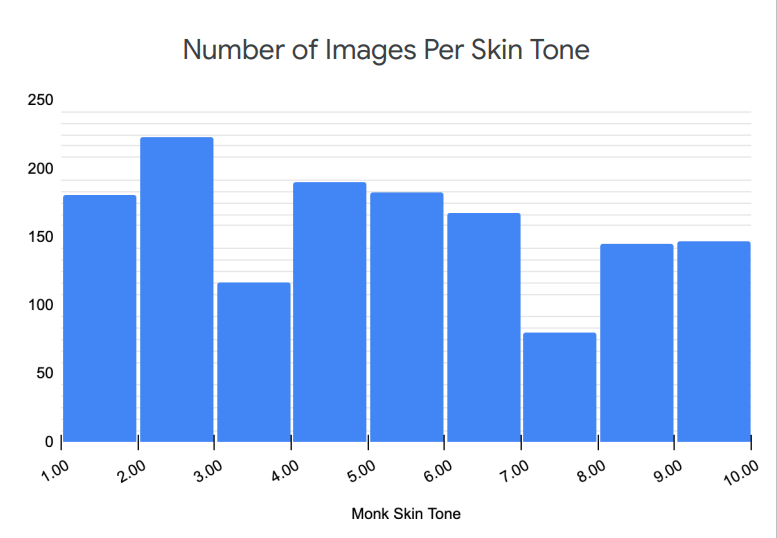
\includegraphics[scale=0.9]{Template_Latex_TCC-UNIFTEC/_lib/imagens/MSTDataset.png}

\label{fig:x MST_Dataset}
\centering{\Fonte{Skin Tone Research} \footnote{https://skintone.google/mste-dataset}}
\end{figure}

Na Figura \ref{fig:x MST_Dataset} demonstra-se a quantidade de imagens por classificação de tom de pele. O conjunto de amostras possui uma distribuição de tons consistentes, contudo os tons 3 e 7 apresentam menos imagens disponíveis. Nota-se que a diferença de quantidade imagens é entorno de 150 imagens entre o tom 2 e 7. Para o trabalho isso não é um impeditivo, pois o \textit{dataset} não é disponibilizado para treinamento de modelo. O \textit{dataset} é utilizada para estudo e verificação dos resultados. Logo, não há interferência no modelo utilizado, apenas dispõe menos exemplos de validação para o tom.


\begin{figure}[h!]
\caption{Exemplos de poses do dataset}
    \label{fig: poses}
    \begin{minipage}[!]{0.55\linewidth}
    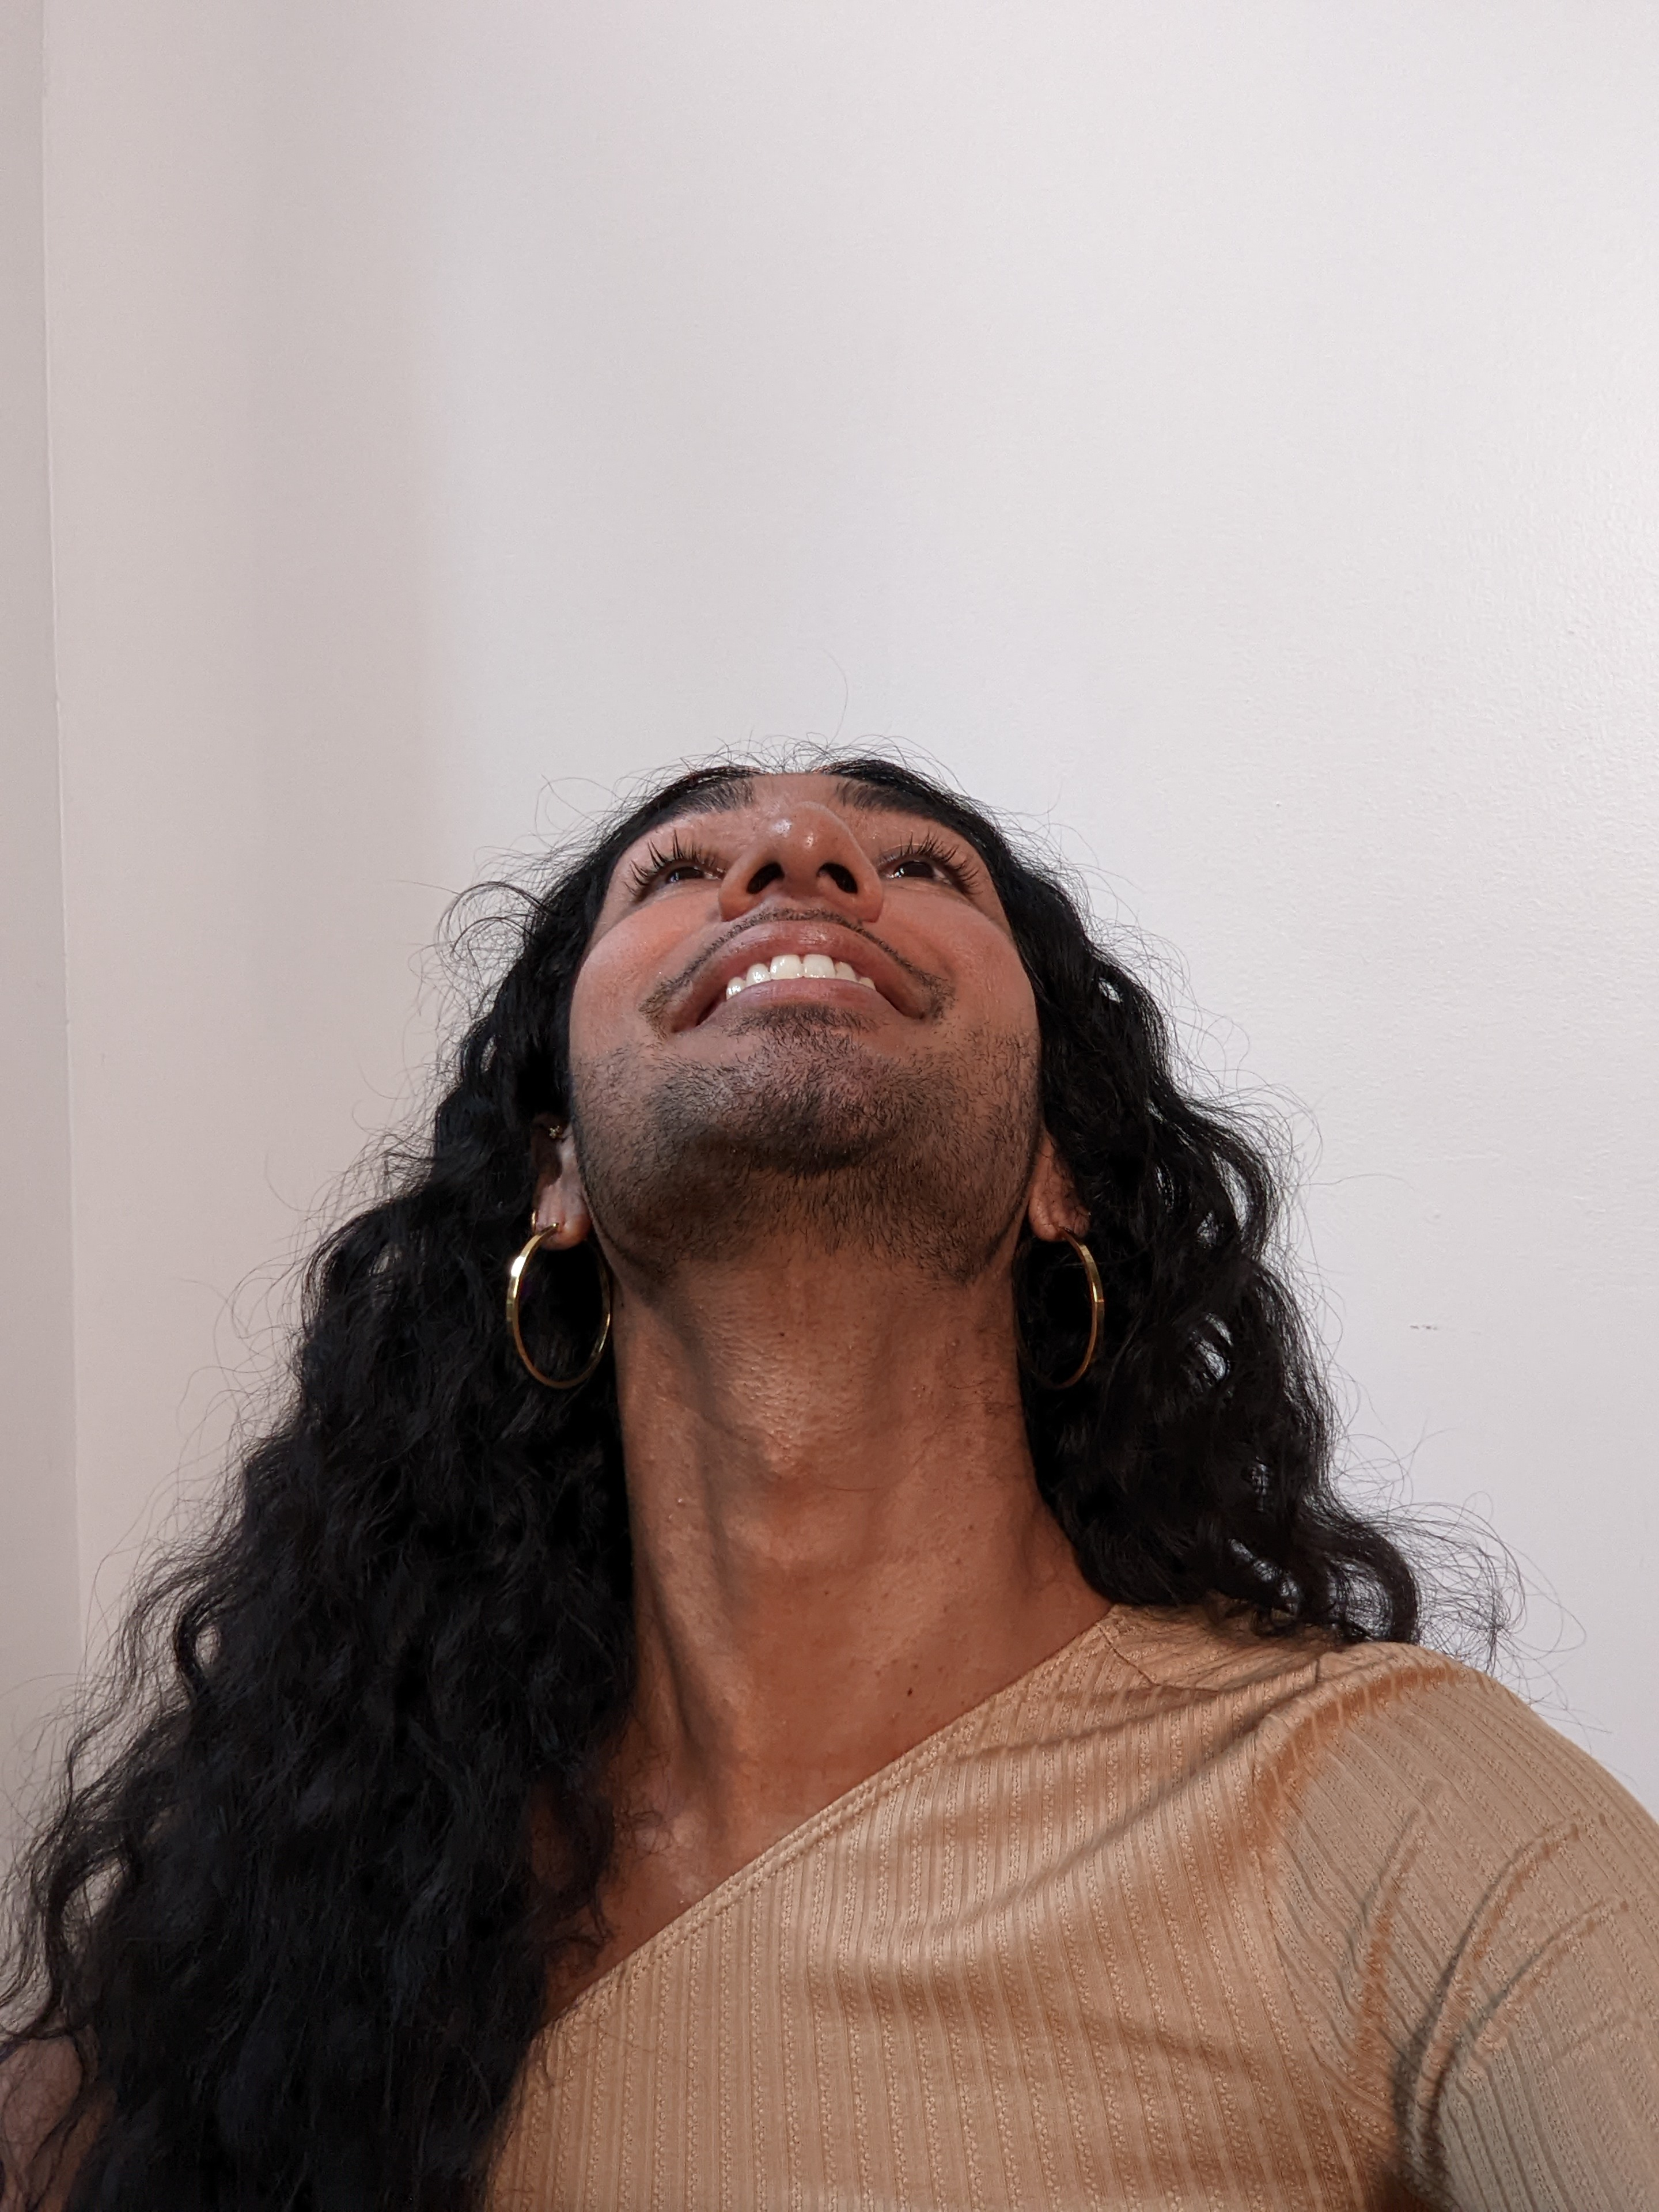
\includegraphics[height=10cm]{Template_Latex_TCC-UNIFTEC/_lib/imagens/bottom.jpg}\\ \centering\textbf{ a) Pose \textit{Bottom}}
    \label{fig: bottom}
    \end{minipage}
    \begin{minipage}[!]{0.55\linewidth}
    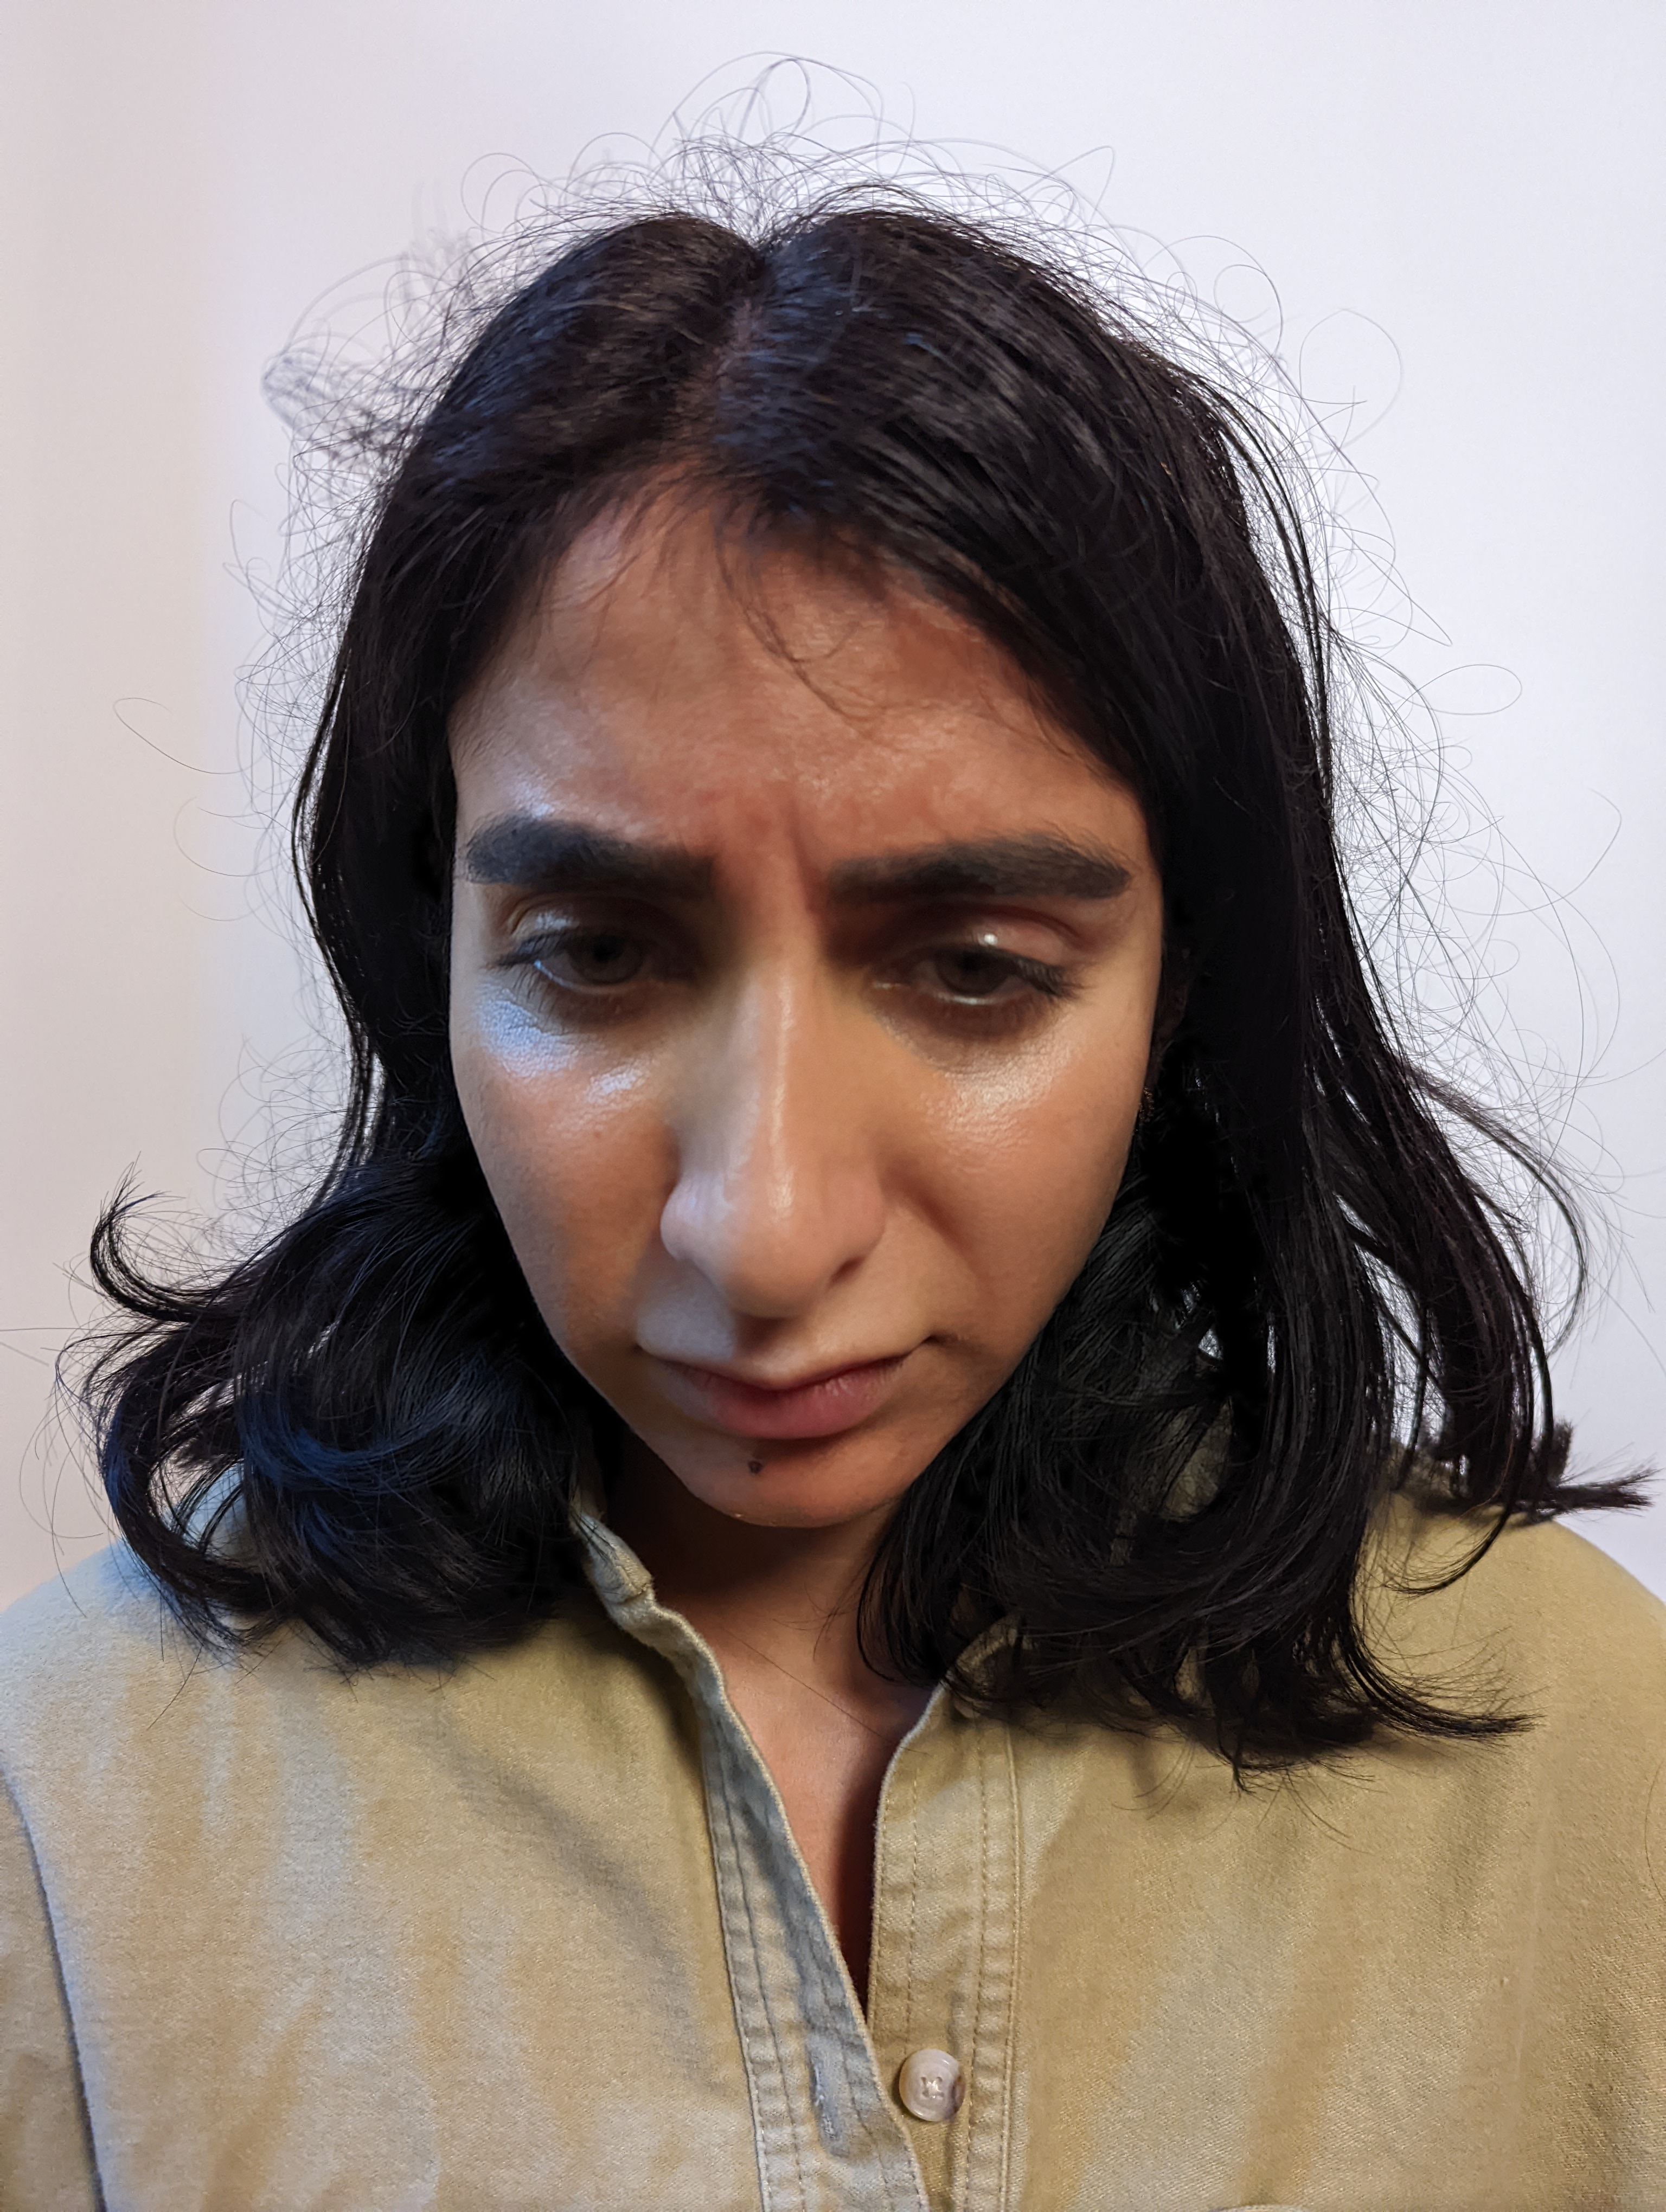
\includegraphics[height=10cm]{Template_Latex_TCC-UNIFTEC/_lib/imagens/frontal.jpg}\\ \centering\textbf{ b) Pose \textit{Frontal}}
    \label{fig: frontal}
    \end{minipage}
    \begin{minipage}[!]{0.55\linewidth}
    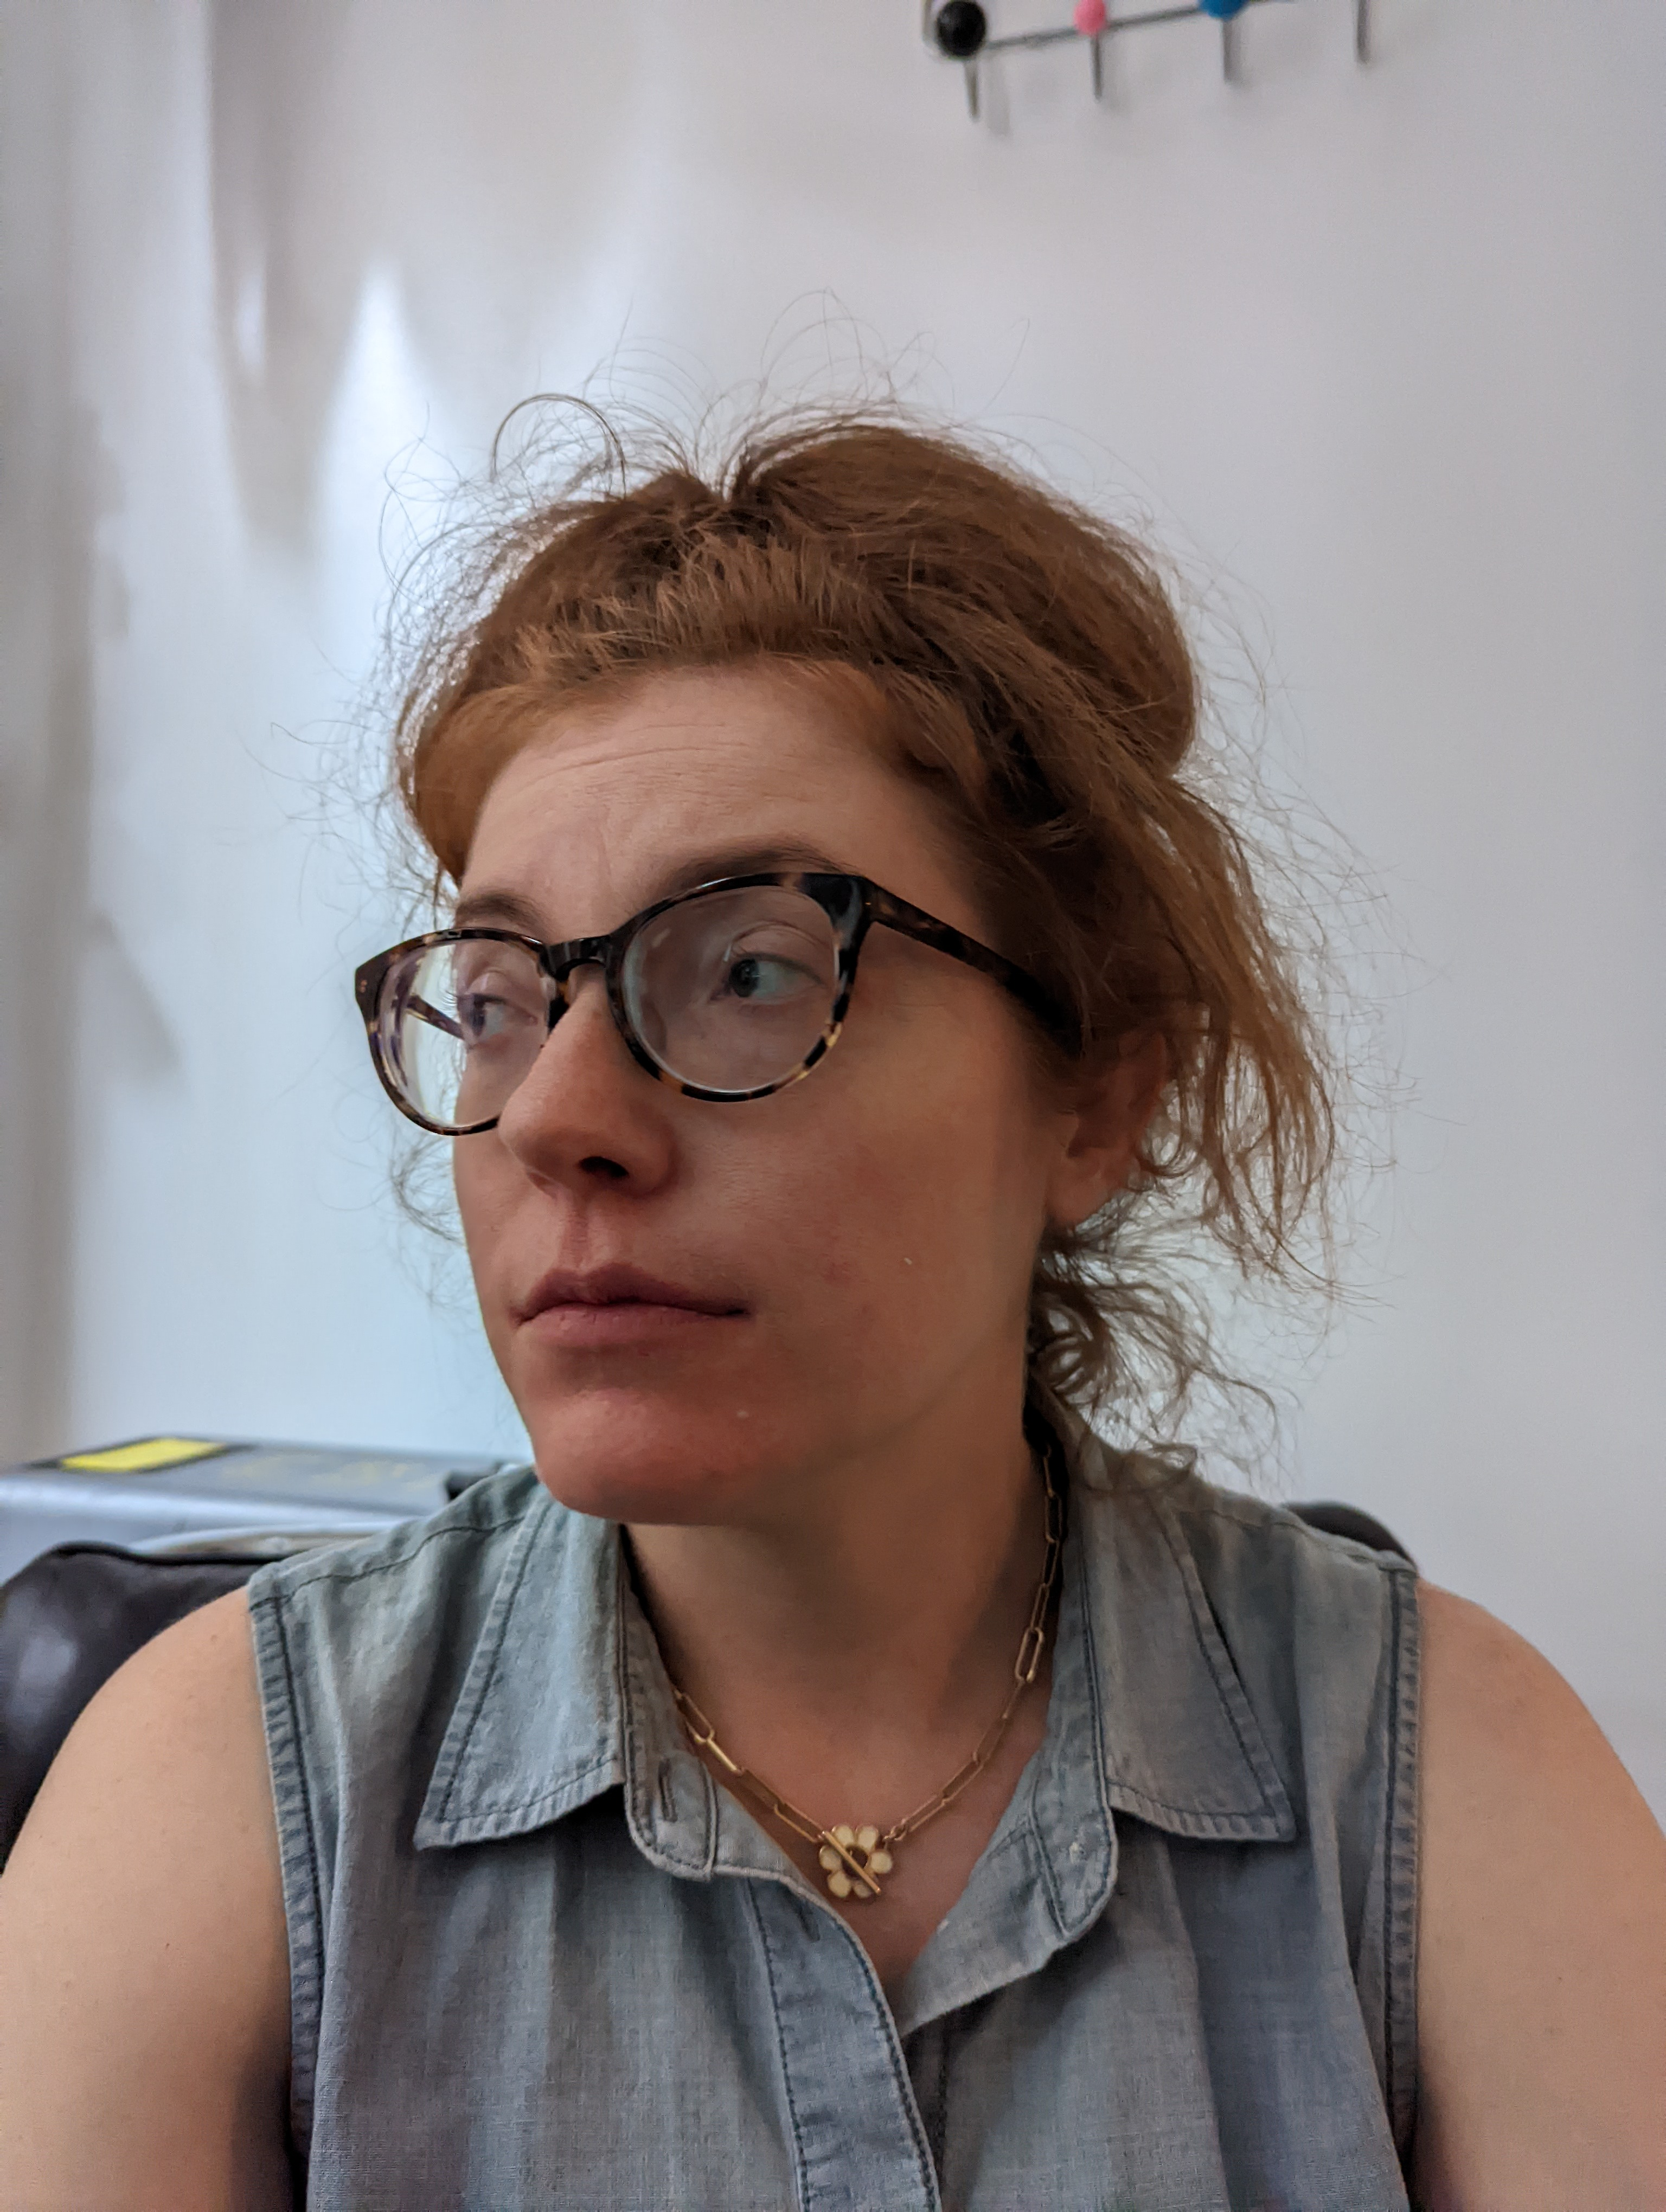
\includegraphics[height=10cm]{Template_Latex_TCC-UNIFTEC/_lib/imagens/side.jpg}\\ \centering\textbf{ c) Pose \textit{Side}}
    \label{fig: side}
    \end{minipage}
    \begin{minipage}[!]{0.55\linewidth}
    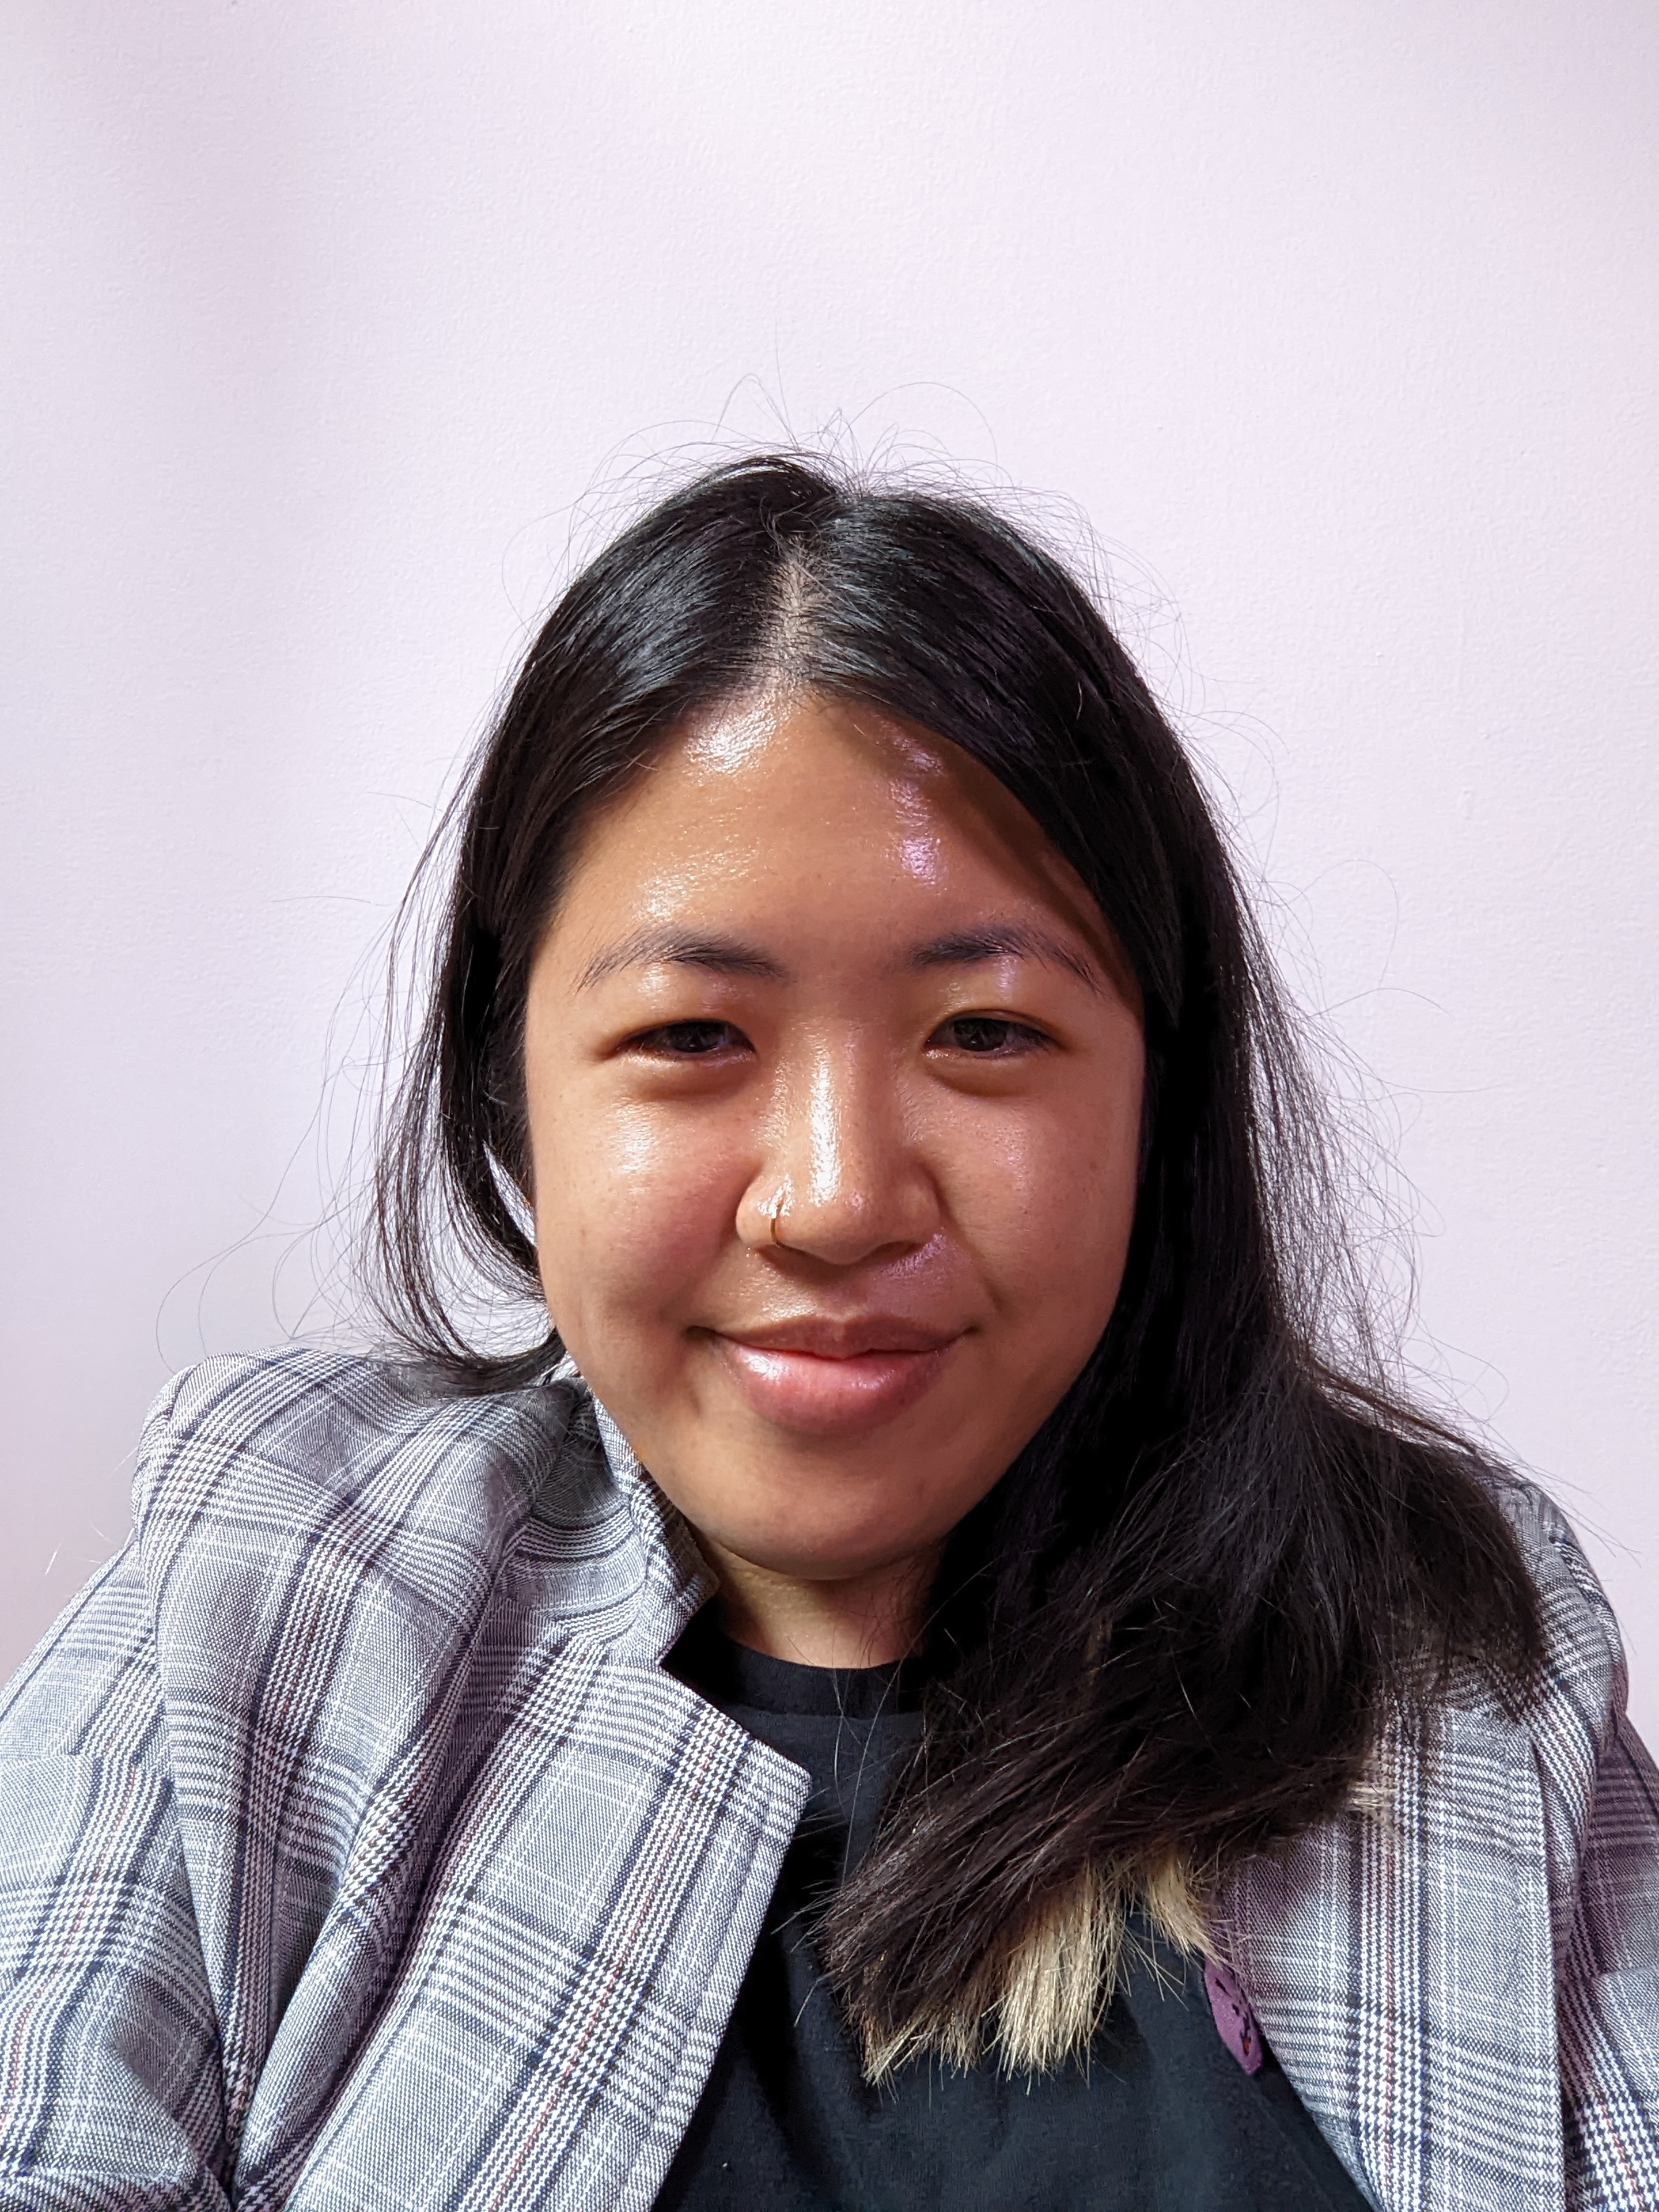
\includegraphics[height=10cm]{Template_Latex_TCC-UNIFTEC/_lib/imagens/facing_camera.jpg}\\ \centering\textbf{ d) Pose\textit{ Facing Camera}}
    \label{fig: facing_camera}
    \end{minipage}
\Fonte{Skin Tone Research} \footnote{https://skintone.google/mste-dataset}
\end{figure}

O \textit{dataset} MST-E possui 1515 imagens com diferentes poses e iluminações nas imagens. Sendo classificadas as poses como \textit{frontal} para pose de frente a câmera como na Figura \ref{fig: frontal}, \textit{bottom} para pose de frente com o queixo para cima como na Figura \ref{fig: bottom}, \textit{side} para pose com o rosto de lado, tanto para lado direito quanto para o lado esquerdo, como na Figura \ref{fig: side} e\textit{facing\_camera} para poses de frente olhando para a câmera como na Figura \ref{fig: facing_camera}, como pode ser visto na Figura \ref{fig: poses}. A quantidade de poses são relativas à escolha dos voluntários, assim como a presença de caretas. Quanto a iluminação, não há parametrização de quão claro ou escura é a iluminação utilizada. Há a classificação de duas diferentes iluminações, sendo elas \textit{poorly\_lit}, para iluminações de baixa qualidade,  e \textit{well\_lit}, para iluminações de boa qualidade. Não há padronização de plano de fundo nas fotos, visto que algumas imagens foram fotografadas ao ar livre. Algumas pessoas utilizam acessórios como máscaras e óculos. As imagens com máscara também foram categorizadas e separadas. Além disso, as imagens são catalogadas por Monk fornecendo os tons de pele verdadeiros do MST.


Para o propósito do trabalho desconsideraram-se os vídeos e as imagens com pessoas utilizando máscara e em pose não frontal. Para isso foi desenvolvido uma automatização como na Figura \ref{fig:x Visual_basic} para excluir os itens não necessários considerando as classificações compartilhadas na documentação do \textit{dataset}. 

\begin{figure}[h!]
\centering
\caption{Desenvolvimento para seleção de imagens relevantes}
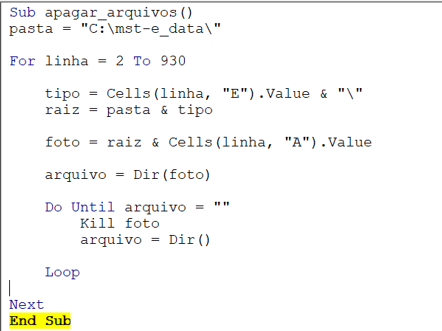
\includegraphics[scale=0.9]{Template_Latex_TCC-UNIFTEC/_lib/imagens/VisualBasic.png}

\label{fig:x Visual_basic}
\centering{\Fonte{Autor}}
\end{figure}

No desenvolvimento demonstrado na Figura \ref{fig:x Visual_basic}, é feito a leitura do arquivo csv disponibilizado pelo arquivo do \textit{dataset} MST-E. O arquivo foi modificado para ter somente as imagens a serem excluídas. No desenvolviwnto é verificao o nome das imagens disponibilizados no arquivo e procurados na pasta informada. O arquivo achado é excluído da pasta. O mesmo processo ocorre até a leitura do csv finalizar.

A partir disso, foi excluído os conteúdos de video e as imagens categorizadas com pose \textit{bottom} e \textit{side}, além das que continham máscara, mantendo as poses \textit{facing\_camera} e \textit{frontal} sem as fotos com máscara. Com isso, foram retiradas 929 arquivos, sendo elas imagens e vídeos não relevantes, totalizando em 617 imagens para estudo. Além disso, 32 imagens foram retiradas por estarem desfocadas e não serem viáveis de avaliação.

\subsection{Ajuste do tamanho da imagem}
Como as imagens possuíam tamanhos diferentes, para deixá-las todas em tamanho padrão utilizou-se a biblioteca OpenCV e o método resize(). O método pretende de redimensionar as imagens na altura, largura e interpolação com liberdade. No desenvolvimento, foi utilizado para ajustar a altura das imagens para 250px e largura para 250px. 

\subsection{Conversão de cores}
Para utilizar algumas funções do OpenCV e ter resultados mais precisos se faz necessário converter as cores das imagens ao longo do processamento. Ao longo do desenvolvimento foram realizadas ao todo 11 conversões de cores nas imagens. Para isso foi utilizada a função cvtColor()\footnote{https://docs.opencv.org/3.4/d8/d01/group__imgproc__color__conversions.html} que possui inúmeras possibilidades de conversão de cores. Cada modelo tem seu cálculo implícito, dependendo do parâmetro utilizado para conversão, mas para a conversão basta a inserção da imagem na função e o parâmetro que define qual sistema de cor está a imagem e para qual sistema deve-se ser convertido. Converteram-se as imagens do modelo de cor BGR para GRAY, BGR para HSV, HSV para BGR, BGR para RGB e BGR para LAB.

Como as imagens inseridas são lidas como BGR e não RGB todas as conversões de imagens partiram de BGR para os modelos de cor utilizados. Assim como para melhor visualização, visto que uma imagem em BGR não apresenta a visualização de cores esperadas originalmente.

Converteram-se as imagens dos modelos BGR para GRAY, para leitura e identificação de características. O modelo GRAY se refere a conversão para tons de cinza. A conversão foi utilizada para seguir o processo de pré-processamento de imagem que requer que a cor esteja em GRAY.

A conversão do sistema de cor BGR para HSV foi necessária para a extração de pele realizada com \textit{threshold} que será descrita ao longo do Capítulo \ref{cap:desenvolvimento}. Assim como a conversão do sistema de cor HSV para BGR para seguir o processo e visualização da imagem durante o desenvolvimento. 

Com relação à conversão do sistema de cor de BGR para LAB foi utilizada para a etapa de validação, onde os resultados foram calculados utilizando valores no modelo CIELab,  será descrita ao longo do Capítulo \ref{cap:desenvolvimento}.


\section{Pré-Processamento de Imagens}
O pré-processamento que se baseia em realizar identificações que facilitam a identificação das áreas relevantes, como a identificação de contornos, bordas e regiões da face como olhos, boca e nariz. Para isso é necessário o desenvolvimento de algumas etapas que serão abordadas ao longo desta seção.

\subsection{Remoção de regiões}
Com a imagem em GRAY, utilizou-se o método CascadeClassifier() para classificação em cascata da OpenCV. Primeiro ,o método CascadeClassifier é criado e o arquivo XML é carregado usando o método CascadeClassifier::load. Posteriormente, a detecção é feita usando o método CascadeClassifier::detectMultiScale, que retorna retângulos de limite para os rostos, boca, nariz ou olhos detectados. 
Para a identificação de regiões, utilizou-se dois arquivos do tipo XML da hospedagem oficial do OpenCV no repositório do GitHub\footnote{https://github.com/kipr/opencv/tree/master/data/haarcascades} modelados para a detecção frontal de face\footnote{https://github.com/kipr/opencv/blob/master/data/haarcascades/haarcascade\_frontalface\_default.xml} e detecção de olhos\footnote{https://github.com/kipr/opencv/blob/master/data/haarcascades/haarcascade\_eye.xml} e dois arquivos do tipo XML para a modelagem de detecção de nariz\footnote{https://github.com/atduskgreg/opencv\-processing/blob/master/lib/cascade\-files/haarcascade\_mcs\_nose.xml} e boca\footnote{https://github.com/atduskgreg/opencv\-processing/blob/master/lib/cascade\-files/haarcascade\_mcs\_mouth.xml} disponibilizados pela comunidade pelo repositório do GitHub \footnote{https://github.com/atduskgreg/opencv\-processing/tree/master/lib/cascade\-files}.
A identificação da face foi utilizada para identificar as faces e remover áreas de não interesse das outras análises. Para as regiões de olhos, boca e nariz, as áreas identificadas 
são pintadas da cor preta para serem desconsideradas, conforme Figura \ref{fig: Etapas_de_teste_roi}.

\begin{figure}[h]
\centering
\caption{Retirada de áreas de influência.(1) Imagem de referência; (2) Imagem de primeiro recorte;  (3) Imagem de exclusão de olhos; (4) Imagem de exclusão de nariz; e, (5) Imagem de exclusão de boca.}
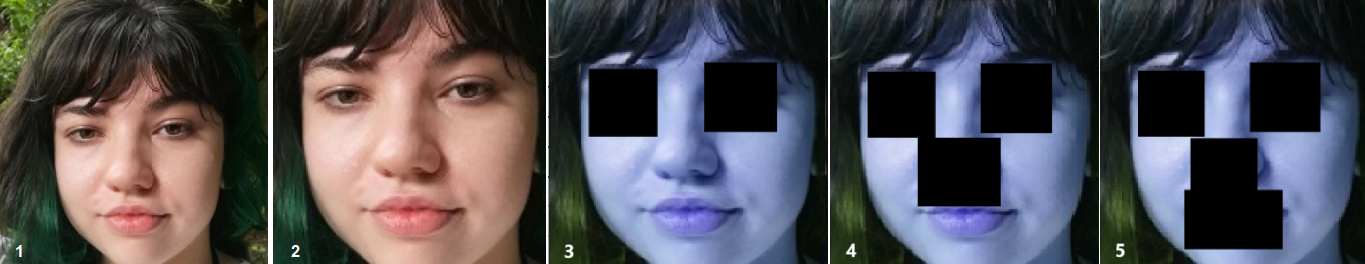
\includegraphics[scale=0.65]{Template_Latex_TCC-UNIFTEC/_lib/imagens/vittoriatestes2.png}

\label{fig: Etapas_de_teste_roi}
\centering{\Fonte{Autor}}
\end{figure}

Na Figura \ref{fig: Etapas_de_teste_roi} (1) demonstra-se a imagem sem tratamento colocado pelo usuário como referência, em seguida a imagem (2) onde é estabelecido o primeiro recorte da identificação do rosto pelo Haar Cascade. Na imagem (3) demonstra-se a exclusão da área dos olhos, por consequência a imagem (4) com a exclusão da região dos olhos e nariz e, por fim, a imagem (5) a exclusão da região dos, olhos, nariz e boca. 
A saída da função é a imagem  em BGR recortada e com as áreas de não interesse excluídas. A imagem então é convertida do modelo BGR para HSV para a extração de pixel de pele e não-pele.

\subsection{Segmentação de pele}

Para a segmentação de pele utiliza-se a função de extração de pele com \textit{threshold}. Para esse processo, cria-se uma imagem binária filtrando pixels com base em um limite definido no espaço de cor HSV. Cada pixel de uma imagem é verificado na faixa de limite, onde os valores limites são os valores HSV que denotam a faixa de tom de pele. O limite mínimo usado se enquadra no \textit{array} de 0, 48, 80 e o limite máximo se enquadra no \textit{array} 20, 255, 255. Para isso utilizou-se o método inRange() da biblioteca OpenCv para fazer a limitação, onde se o pixel lido estiver na faixa dos mínimos, torna-se o branco, se não, preto.

Em seguida, é utilizado o método GaussianBlur() da biblioteca OpenCV para suavização do resultado. Neste método é utilizado um kernel gaussiano e para isso especifica-se os valores de largura e altura do kernel. Também deve-se especificar o desvio padrão nas direções X e Y, sigmaX e sigmaY respectivamente. O desfoque gaussiano visa retirar o ruído da imagem, sendo uma variação dos valores nos níveis de cinza dos pixels na imagem, causados por erros na transmissão de dados, ou eventuais distorções causadas na fase de aquisição de uma imagem em geral. A função é dada como altamente eficaz na remoção do ruído gaussiano de uma imagem, por este motivo foi utilizado. Para isso, os parâmetros utilizados foram o resultado da imagem criada a partir do processamento de \textit{threshold}, valor de X e Y como 0, sendo os valores calculados a partir dos valores de sigma colocados, valores de 3 de sigmaX e sigmaY e borda padrão como 0.

Após a suavização, utilizando da biblioteca OpenCV, é executado o método bitwise\_and(). O método tem como objetivo obter a imagem final subtraída da imagem binária, resultando na imagem final convertida do espaço de cor HSV para BGR. O método bitwise\_and() visa a extração bit a bit de qualquer parte de uma imagem. E neste caso, utiliza-se o método para remover os pixel pretos tendo como parâmetros as imagens sem tratamento e a imagem gerada a partir do filtro de Gaussiana, tendo como resultado imagens como a Figura \ref{fig: Etapas_threshoding}. 

\begin{figure}[h]
\centering
\caption{Etapas de desenvolvimento. (1) Imagem de referência; (2) Imagem com recorte na face; e, (3) Remoção de pixel com Thresholding}
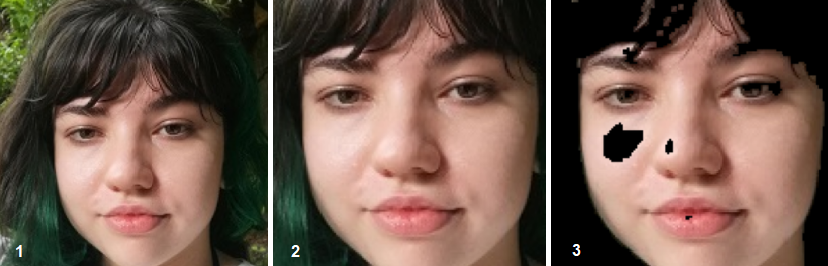
\includegraphics{Template_Latex_TCC-UNIFTEC/_lib/imagens/vittoriatestes.png}

\label{fig: Etapas_threshoding}
\centering{\Fonte{Autor}}
\end{figure}

A Figura \ref{fig: Etapas_threshoding} representa o resultado do processo de \textit{thresholding} isoladamente para melhor visualização. Nela foram ignorados a análise resultante utilizando a extração de regiões para representar apenas o resultado do processo de \textit{thresholding}. A imagem 1 representa a entrada original da imagem no sistema, a imagem 2 representa o recorte da imagem localizando a face e a imagem 3 o resultado das três etapas de \textit{ threshold} sendo limitação, suavização, subtração da imagem binária, demostrados todos no espaço RGB. Contudo, como saída do desenvolvimento da segmentação de pele temos uma imagem HSV que passa pela conversão para BGR.

\subsection{Seleção da cor dominante}
A extração de cores é executada utilizando o método Kmeans. O desenvolvimento utiliza uma cópia da imagem que está sendo a analisada e converte de BGR para RGB. A imagem convertida é reorganizada utilizando o método reshape(). O método reshape() tem o papel de mudar o formato do \textit{array} sem mudar o conteúdo
O método Kmeans verifica uma imagem no sistema de cor RGB e tem como parâmetro a quantidade de \textit{clusters} utilizados, a  geração de números aleatórios para inicialização do centroide como nulo e o número de vezes que o algoritmo k-means é executado com centroides diferentes, determinado como automático.

Após a extração de cores seleciona-se a cor dominante com a verificação de pixel por pixel. A quantidade de ocorrência de cores é verificada, sendo somado a quantidade de pixels da mesma cor. As cores mais comuns encontradas são reorganizadas em sequência crescente de quantidade ocorrência para identificação da cor mais dominante.Além de ser efetuado o cálculo de percentagem relativa a sua proporção.

 
\section{Resultado visual}
Para fins visuais é criada uma barra de cores para visualização das cores dominantes encontradas. As cores analisadas com as suas respectivas percentagens são adicionadas em um \textit{array}. Os valores de porcentagem são organizados de forma decrescente. Sendo, a primeira cor, a esquerda, adicionada na barra, a cor com a maior porcentagem. Por consequência, a cor mais dominante. Criando-se a imagem com as respectivas cores encontradas e a demonstração visual da quantidade percentual encontrada, conforme Figura \ref{fig:x Paleta_resultante}.  

\begin{figure}[h]
\centering
\caption{Paleta resultante}

\includegraphics{Template_Latex_TCC-UNIFTEC/_lib/imagens/paleta.png}

\label{fig:x Paleta_resultante}
\centering{\Fonte{Autor}}
\end{figure}


\section{Validação}
Para validação de resultados comparou-se os valores categorizados por Monk aos resultados alcançados pelo desenvolvimento. Utilizando a biblioteca Scikit-image e o método deltaE\_ciede2000(). O método baseia-se em comparar duas cores no sistema de cor CIELab. Para isso foi feita a conversão do sistema de cor BGR para Lab.

No desenvolvimento, utilizou-se os 10 tons da paleta de Monk disponibilizados no modelo CIELab presentes da documentação da paleta\footnote{https://skintone.google/get-started}. O método requer a inserção de duas várias com o valor de cor CIELab, fator de luminosidade (kL), fator de cromaticidade (kC), fator de escala de matiz (kH) e de canais com valores padrões. No desenvolvimento utilizou como referência a cor disponibilizada pela paleta de Monk e a cor de comparação a cor dominante encontrada. Os demais parâmetros utilizaram do valor padrão igual a 1

Se realizaram três analises diferentes e os resultados foram salvos na planilha csv criada. Na primeira análise é realizada o cálculo CIEDE2000 para todos os tons de MST. Nisso a análise baseia-se na comparação de valores das 10 cores MST com a cor dominante, sendo os 10 valores salvos em uma lista. Esses valores são analisados e verificados com o método min() para trazer o valor de distância mínima, sendo o valor ideal esperado de todos os valores que constam na lista, sendo salvo no arquivo csv como mínimo\_lab. 

A segunda análise se baseia em selecionar o valor de categorização MST conforme o valor mínimo encontrado. Para isso utiliza-se o método index() para selecionar a posição na lista em que se encontra o valor mínimo encontrado anteriormente. Este valor é salvo no arquivo csv como classificacao\_indicada\_lab. Para a terceira análise, utilizando a cor classificada por Monk e a cor dominante encontrada, se refaz o cálculo com o método deltaE\_ciede2000() para calcular o valor verdadeiro de acordo com Monk. Ou seja, é apenas avaliado a cor classificada por Monk e a cor encontrada tendo como resultado a distância a qual não é necessariamente a menor entre todas as cores, sendo este valor salvo no arquivo csv como distancia\_lab.

Em conclusão é feito o cálculo de acurácia conforme realizado no artigo \cite{Classification_Algorithm_for_Skin_Color_CASCo_A_new_tool} . O cálculo de baseia em subtrair de 100 o valor de minimo\_lab. 

Após o processamento, salvam-se as informações de nome de arquivo, pose, característica de iluminação, tom MST, o tom encontrado em CIELab, a distância mínima ideal, a distância encontrada e a acurácia em um arquivo do tipo csv.

Criação de arquivo csv para estudo e comparação de resultados. Cada imagem analisada tem seus dados salvos para verificação dos resultados em um arquivo criado durante o processamento. Como as imagens do \textit{dataset} já foram categorizadas por Dr. Monk as informações que constam no de nome da imagem apenas para referência, número de objeto estudado, pose utilizada, descrição de luz e a classificação mst são extraídos e salvos no arquivo csv. Além disso, são adicionadas as informações CIELab do tom MST e os valores resultantes do desenvolvimento como a cor dominante em CIELab, a menor distância calculada encontrada entre todas as cores da paleta para CIELab, a distância resultante encontrada entre a cor dominante CIELAB e o tom classificado, a classificação indicada conforme a distância resultante e a acurácia.

A criação do arquivo se dá com a função open() da biblioteca CSV. A função permite criação, escrita, leitura e modificação de arquivo. No desenvolvimento foi utilizada a função open() para criar o arquivo local  como o modo 'w' e modificá-lo como o modo 'a'.

O método DictWriter() foi utilizado para criar o cabeçalho com as informações \textit{'image\_name', 'subject','pose', 'light', 'MST','LAB','distancia_lab', 'minimo\_lab', 'classificacao_indicada_lab', 'acuracia'} e seu demilitado sendo uma vírgula. Para adicioná-lo ao arquivo criado utilizou-se o método writerheader() para adicioná-lo ao arquivo.

Para a modificação do arquivo csv, o arquivo é reaberto para modificação e com o método writer() e writerow() é adicionado uma nova linha ao arquivo à cada imagem processada.

% \section{Considerações finais}
	\chapter{Experimentos e Resultados}
\label{cap:experimentos-resultados}
%Este capítulo visa apresentar os testes executados durante o estudo e elaboração deste documento, assim como os resultados alcançados durante a construção. Abordar os principais pilares para a execução do desenvolvimento e verificação de validação dos testes para alcançar os objetivos do projeto. O desenvolvimento visou trabalhar a partir um escopo menor e ampliar posteriormente.

Três classificadores foram analisados para a identificação facial, sendo elas o Haar Cascade, histogramas e redes neurais convolucionais. As três opções são amplamente utilizadas para na área de reconhecimento facial. Neste caso, foi optado por utilizar o classificador Haar Cascade pela facilidade de utilização e de identificação de diferentes características que planejou-se eliminar durante a manipulação das imagens, com pouca necessidade de codificação. Neste caso, não foi considerado relevante o tempo de processamento das imagens e não foi avaliado os resultados de precisão que os modelos obtivessem. 

Para os experimentos de tratamento de imagem foram utilizados imagens diferentes disponibilizadas na internet escolhidas para compreender cenários diversos. Esses experimentos tinham como intuito verificar enquadramento e exclusão de regiões sem presença de pele humana em situações não controladas a fim de entender o comportamento a serem tratados. Os cenários escolhidos tratavam-se de imagens onde havia apenas uma pessoa por foto, onde a pessoa fotografada constava com o rosto angulado, com cabelo na frente do rosto e o fundo da foto com cores próximas a tons de pele, sem controle de iluminação. 

Com essas imagens foram executados testes de dimensionamento para identificação de rosto utilizando Haar Cascade. Por utilizar o Haar Cascade com treinamento para localização de rostos frontais, os testes resultaram apontaram para o uso de imagens com o rosto em posição frontal e com menor angulação possível. Também percebeu-se que o cabelo frente ao rosto não era excluído completamente durante o processamento da imagem, além da sombra que o cabelo causava influenciar no resultado de identificação de cores. Ademais, as cores de fundo das imagens não demonstraram influenciar nos resultados nos testes avaliados. Também percebeu-se que a identificação de tom de pele dominante nas imagens eram influenciados pelas regiões da face como o nariz, olhos, sobrancelha e boca, pela presença de sombreamento e a presença de pelos. 

A partir disso, baseado nos resultados dos testes do classificador, escolheu-se recortar as imagens onde o algoritmo identificou a face para minimizar influência de cabelo e de objetos. Após o foco na face, retirou-se a região dos olhos na imagem e verificou-se novamente os resultados da paleta dominante. Realizou-se o mesmo para a região do nariz e boca como pode ser visto na Figura \ref{fig: Etapas_de_teste_roi}.

As áreas excluídas são identificadas com Haar Cascade, cada área com seu modelo próprio de identificação, e pintadas de preto para retirada dos pixels. A retirada das áreas melhorou a percepção de coloração dominante na paleta resultante e aumentou a presença de cores mais próximas à paleta de Monk.

Com base no estudo \cite{Automatic_Skin_Tone_Extraction_for_Visagism_Applications} e a Tabela \ref{table:Tabela_comparativa_sistemas_de_cores} optou-se por utilizar um sistema de cor com bom desempenho individual. Como o sistema de cor HSV e YCrCb obtiveram resultados semelhantes, foi avaliado o comportamento de ambos sistemas nas fotos utilizadas anteriormente. O teste constituía em avaliar as imagens e verificar a distinção do uso do modelo HSV e YCrCb na identificação de pixel relevantes. Os testes obtiveram resultados semelhantes, como esperado, contudo o modelo HSV comparado ao modelo YCrCb trouxe mais definição de detalhes, o que pode ser verificado na Figura \ref{fig:x Etapas_de_teste_cores}.

\begin{figure}[h]
\centering
\caption{Comparação de resultados entre HSV e YCbCr. (1) Imagem de referência; (2) Imagem com HSV; e, (3) Imagem com YCbCr.}
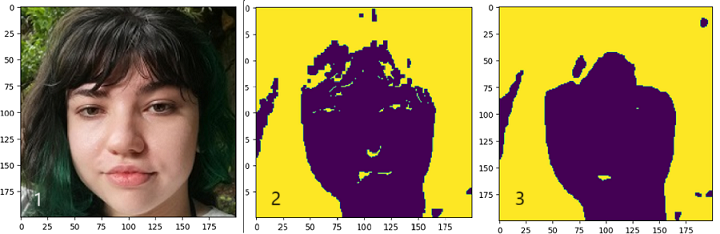
\includegraphics[scale=1.2]{Template_Latex_TCC-UNIFTEC/_lib/imagens/testHsvYcbcr.png}

\label{fig:x Etapas_de_teste_cores}
\centering{\Fonte{Autor}}
\end{figure}


Na Figura \ref{fig:x Etapas_de_teste_cores} a imagem (1) representa a imagem de referência, a (2) o resultado utilizando sistema de cor HSV e a imagem (3) o resultado utilizando o modelo YCbCr. Nota-se que no teste ambos sistemas distinguiram a região da face, contudo o modelo HSV retorna mais detalhes faciais comparado ao modelo YCbCr, o que pode auxiliar na identificação de pixels não relevantes na face, visto que o intuito é apenas o tom de pele.

Para a identificação dominante de tom de pele utilizando Kmeans avaliou-se alterar o parâmetro de n\_clusters. O parâmetro detém o valor de número de \textit{clusters},  assim como o número de centroides a ser utilizado. Em suma, o valor utilizado retorna a quantidade de cores identificadas por conjunto. Com isso, avaliou- se utilizar 1 a 10 , 15 e 20 \textit{clusters} nas imagens do \textit{dataset} MST-E para verificar qual configuração de \textit{clusters} retorna valores mais precisos. 

Com os testes com as 585 imagens do \textit{dataset} notou-se que a quantidade de \textit{cluster} não está relacionada a melhora na identificação da cor dominante. Utilizar menos \textit{clusters} na análise não trazem valores de cor dominantes mais próximas a cores da paleta de Monk, assim como utilizar mais \textit{clusters} não trazem melhores resultados. Além disso, para algumas imagens diferentes \textit{clusters} traziam os mesmos resultados de identificação. Contudo, nos testes utilizando 1, 2 e 3 \textit{clusters} algumas imagens não obtiveram resultado de cor dominante identificada sendo desconsiderados utilizar os \textit{clusters}. 

Além disso, para a validação de resultados de identificação de tom de pele dominante analisou-se duas formas diferentes para calcular a distância entre os tons da paleta de Monk e os tons dominantes encontrados. Na primeira avaliação, utilizou-se a distância euclidiana com o modelo RGB. Na segunda avaliação, utilizou-se a distância Delta E 2000 com o modelo CIELab que pode ser visto na Tabela \ref{table:Tabela_comparativa_entre_os_clusters_e_modelo_rgb} para o modelo RGB e a Tabela \ref{table:Tabela_comparativa_entre_os_clusters_e_modelo_cielab} para  modelo CIELab.

% \begin{table}[]
% \centering
% \caption{Tabela comparativa entre os clusters e modelos de cor}
% \label{table:Tabela_comparativa_entre_os_clusters_e_modelo}\textbf{}
% \resizebox{\columnwidth}{!}{%
% \begin{tabular}{lllllllll}
% \hline
% Clusters & RGB & \textgreater{}=1 & \textgreater{}=2 & \textgreater{}=3 & CIELab & \textgreater{}=1 & \textgreater{}=2 & \textgreater{}=3 &  \\ \hline
% 4        & 82  & 179              & 269              & 336              & 82     & 179              & 248              & 352              &  \\ 
% 5        & 68  & 180              & 270              & 329              & 75     & 174              & 259              & 347              &  \\ 
% 6        & 64  & 185              & 272              & 329              & 83     & 177              & 263              & 360              &  \\ 
% 7        & 67  & 182              & 265              & 330              & 80     & 173              & 256              & 352              &  \\ 
% 8        & 59  & 181              & 258              & 319              & 85     & 181              & 260              & 352              &  \\ 
% 9        & 65  & 171              & 262              & 322              & 82     & 181              & 263              & 342              &  \\ 
% 10       & 61  & 179              & 266              & 326              & 79     & 179              & 265              & 341              &  \\ 
% 15       & 69  & 180              & 269              & 328              & 84     & 187              & 266              & 349              &  \\ 
% 20       & 67  & 179              & 265              & 327              & 78     & 169              & 256              & 346              &  \\ \hline
% \end{tabular}%
% }
% \centering{\Fonte{Autor}}
% \end{table}

\begin{table}[h!]
\centering
\caption{Tabela comparativa entre os clusters e modelo RGB}
\label{table:Tabela_comparativa_entre_os_clusters_e_modelo_rgb}\textbf{}
\begin{tabular}{lllll}
\hline
Clusters & RGB & =1 &             =2 &             =3                \\ \hline
4        & 82  & 179              & 90               & 67            \\ 
5        & 68  & 180              & 90               & 59            \\ 
6        & 64  & 185              & 87               & 57            \\ 
7        & 67  & 182              & 83               & 65            \\ 
8        & 59  & 181              & 77               & 61            \\ 
9        & 65  & 171              & 91               & 60            \\ 
10       & 61  & 179              & 87               & 60            \\ 
15       & 69  & 180              & 89               & 59            \\ 
20       & 67  & 179              & 86               & 62            \\ \hline
\end{tabular}%
\centering{\Fonte{Autor}}
\end{table}%418

\begin{table}[h!]
\centering
\caption{Tabela comparativa entre os clusters e modelos CIELab}
\label{table:Tabela_comparativa_entre_os_clusters_e_modelo_cielab}\textbf{}
\begin{tabular}{lllll}
\hline
Clusters & CIELab & =1 &            =2 &                =3              \\ \hline
4        & 82     & 179              & 69               & 104           \\
5        & 75     & 174              & 85               & 88             \\ 
6        & 83     & 177              & 86               & 97             \\ 
7        & 80     & 173              & 86               & 96             \\ 
8        & 85     & 181              & 79               & 92             \\ 
9        & 82     & 181              & 82               & 79             \\ 
10       & 79     & 179              & 86               & 76             \\ 
15       & 84     & 187              & 79               & 83             \\ 
20       & 78     & 169              & 87               & 90             \\\hline
\end{tabular}%
\centering{\Fonte{Autor}}
\end{table} %437

Nos testes de validação de modelo das 595 imagens do \textit{dataset}, com o modelo RGB, conforme a Tabela \ref{table:Tabela_comparativa_entre_os_clusters_e_modelo_rgb} utilizar 4 \textit{clusters} retorna melhor desempenho para resultados iguais ao de Monk, contudo 4 \textit{clusters}, 82 imagens obtiveram os valores de classificação igual à classificação de Monk, enquanto 179 imagens tiveram diferença de um tom mais claro ou mais escuro na paleta de MonK, 90 imagens foram classificadas dois tons mais claros ou mais escuros do que a classificação de Monk e 67 imagens foram classificadas com 3 tons mais claros ou mais escuros. Os outros \textit{clusters} tiveram um desempenho significativamente menor considerando as classificações iguais.

Para o modelo CIELab, o melhor desempenho se demonstrou utilizando 8 \textit{clusters}. Sendo 85 imagens classificadas com o mesmo tom do que a classificação de Monk, 181 imagens classificadas com um tom mais claro ou mais escuro, 79 imagens classificadas dois tons mais claros ou mais escuro e 92 imagens classificadas com três tons mais claros ou mais escuros à classificação de Monk. 

Utilizar o modelo CIELab retornou resultados mais próximos à classificação de Monk no consistentemente entre os clusters comparado ao modelo RGB. Sendo o melhor resultado utilizar 8 \textit{clusters}. Sendo, 60,17\% das imagens com resultados próximos ao esperado. Por isso, decidiu-se utilizar o modelo CIELab para a validação de resultados e 8 \textit{clusters} na configuração do Kmeans.

Para fins de estudo e comparação de funcionamento, foi realizado testes de comparação entre paletas utilizando o sistema Casco e as imagens previamente selecionadas. Realizou-se uma comparação de resultados de cor dominante como pode ser visto na Figura \ref{fig:x PerlavsMonk} e por consequência a classificação de tom utilizando a paleta Monk e o programa desenvolvido com a paleta PERLA no artigo \cite{Classification_Algorithm_for_Skin_Color_CASCo_A_new_tool}

\begin{figure}[h]
\centering
\caption{Comparação de classificação paleta PERLA e Monk usando CASCo (1) Classificação PERLA; e, (2) Classificação Monk}
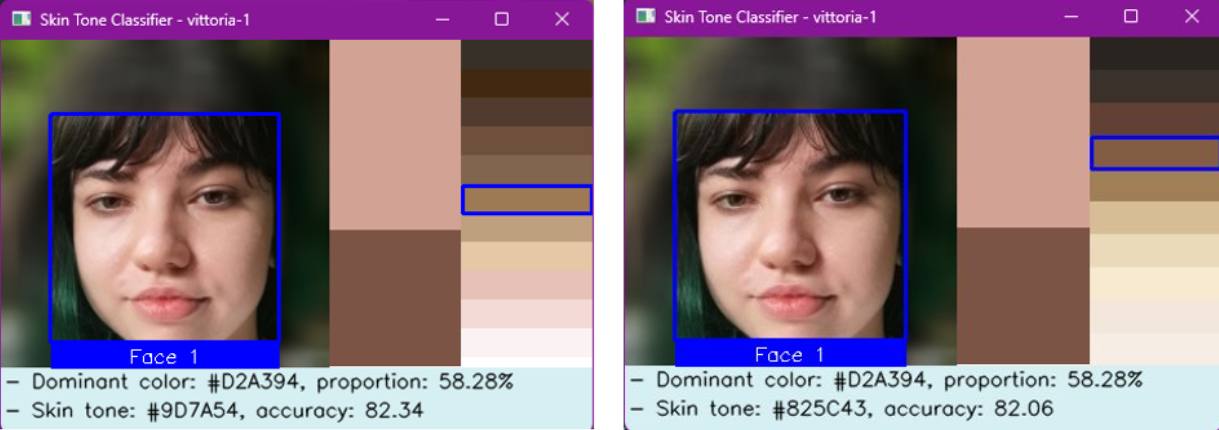
\includegraphics[scale=0.75]{Template_Latex_TCC-UNIFTEC/_lib/imagens/perlavsmonk.png}

\label{fig:x PerlavsMonk}
\centering{\Fonte{Autor}}
\end{figure}

Na Figura \ref{fig:x Etapas_de_teste_cores} a imagem (1) representa o teste utilizando o algoritmo CASCo com a paleta PERLA e a (2) representa o teste utilizando o algoritmo CASCo com a paleta de Monk. Os testes tinham intuito de entender o comportamento do algoritmo. O resultado comparativo destaca que na paleta de Monk o tom classificado ficou mais escuro comparado a paleta PERLA, apesar de ambas terem a mesma cor dominante selecionada. O que está relacionado a distribuições de tons entre as paletas. 
	% ----------------------------------------------------------
% Conclusão
% ----------------------------------------------------------
\chapter{Considerações Finais}
\label{cap:conclusao}
	%\input{elementos-textuais/teste.tex}
    %Elementos pós-textuais
    
    \postextual %
    \bibliography{elementos-pos-textuais/referencias}
%%    \imprimirglossario	
\end{document}


